\documentclass[12pt, a4paper, oneside]{report}

% ── Packages ─────────────────────────────────────────────────────────────────
\usepackage[T1]{fontenc}
\usepackage[utf8]{inputenc}
\usepackage{lmodern}
\usepackage[margin=3.2cm, top=3.0cm, bottom=3.0cm]{geometry}
\usepackage{graphicx}
\usepackage{xcolor}
\usepackage{hyperref}
\usepackage{amsmath}
\usepackage{amssymb}
\usepackage{listings}
\usepackage{xcolor}
\usepackage{booktabs}
\usepackage{array}
\usepackage{microtype}
\usepackage{setspace}
\usepackage{parskip}
\usepackage{fancyhdr}
\usepackage{titlesec}
\usepackage{tocloft}
\usepackage{caption}
\usepackage{subcaption}
\usepackage{float}
\usepackage{enumitem}
\usepackage{url}

\onehalfspacing

% ── Hyperref setup ───────────────────────────────────────────────────────────
% \hypersetup{
%   colorlinks=true,
%   linkcolor=thesisblue,
%   citecolor=thesisblue,
%   urlcolor=thesisblue,
%   pdftitle={VirtioFS Driver for IncludeOS},
%   pdfauthor={Master's Thesis},
% }

\lstdefinestyle{chstyle}{%
basicstyle=\ttfamily\small,
keywordstyle=\color{magenta!100},
tabsize=4,
commentstyle=\color{magenta!100},
frame=tblr
}

% ── Listings style ───────────────────────────────────────────────────────────
\lstdefinestyle{chstyle}{
basicstyle=\ttfamily\small,
keywordstyle=\color{magenta!100},
tabsize=4,
commentstyle=\color{magenta!100},
frame=tblr
}

% ── Caption style ────────────────────────────────────────────────────────────
% \captionsetup{font=small, labelfont={bf,color=thesisblue}, textfont=it}

% ── Graphics path ────────────────────────────────────────────────────────────
\graphicspath{{./diagrams/}{./plots/}}

\title{VirtioFS in IncludeOS \\ 
{\Large University of Oslo}}
\author{Torgeir Skovholt}
\date{\today}

% ════════════════════════════════════════════════════════════════════════════
\begin{document}
\maketitle

% ── Abstract ─────────────────────────────────────────────────────────────────
\chapter*{Abstract}

This thesis presents the design, implementation, and performance evaluation of a
VirtioFS file-system driver for IncludeOS, a unikernel operating system.
VirtioFS enables a Linux host to share a directory with a guest virtual machine
over the FUSE protocol transported via Virtio virtqueues.  Implementing VirtioFS
in IncludeOS required a redesign of the existing virtual filesystem (VFS)
architecture to support clean integration of alternative file-system drivers,
followed by implementation of a Virtio PCI transport layer and a VirtioFS device
driver.

Controlled microbenchmarks comparing the IncludeOS VirtioFS driver against a
Linux guest running under the same QEMU/KVM infrastructure show that IncludeOS
achieves substantially higher I/O throughput across all access patterns.  In
polling mode, peak sequential read throughput reaches 4{,}786~MiB/s ---
a \(\times\)1.74 speedup over Linux POSIX --- with up to \(\times\)3.02 at
small 8~KiB chunk sizes where per-request overhead dominates.  An investigation
of io\_uring SQPOLL as a Linux-side optimisation reveals a counterintuitive
regression of 9--38\% relative to plain POSIX I/O.

An end-to-end video decoding benchmark using the C63 educational codec shows that the I/O throughput advantage translates into a 22.7\% reduction in wall-clock decode time, and eliminates the 25.3\% cold-start penalty observed on Linux.  These results validate the hypothesis that removing general-purpose OS abstractions --- system calls, the VFS, FUSE framing, and a user-space daemon --- yields measurable I/O performance improvements that propagate to realistic application workloads.

% ── Table of Contents ────────────────────────────────────────────────────────
\tableofcontents

% ── Main Matter ──────────────────────────────────────────────────────────────
\pagenumbering{arabic}

% ════════════════════════════════════════════════════════════════════════════
%  CHAPTER 1 — MOTIVATION
% ════════════════════════════════════════════════════════════════════════════
\chapter{Motivation}
\label{chap:motivation}

The project started with a project listing issued by my supervisor regarding
implementing a Virtio file system (VirtioFS) driver in IncludeOS, a unikernel
operating system.  Unikernels are libraries that can be linked with application
code forming an application capable of running directly on bare metal.  A
unikernel executes entirely in kernel mode, thereby eliminating context switch
overhead present in operating systems such as Linux.  This realization motivated
an investigation into whether a VirtioFS driver implemented in IncludeOS could
achieve higher performance than its Linux counterpart, particularly with respect
to IO throughput.

File system support in IncludeOS comprises a virtual file system (VFS) layer,
file descriptor abstractions, incomplete FAT16 and FAT32 drivers, and Virtio and
memory disk block drivers.  The VFS layer is tightly coupled with FAT, hindering
clean integrations of alternative file systems such as VirtioFS.  Therefore, a
redesign of the VFS architecture is necessary to enable clean integration of
alternative file systems.  Developing block-level file system drivers is complex
and prone to errors.  A VirtioFS implementation addresses this by delegating file
system operations to a file system server that performs system calls through the
host kernel, thereby leveraging the host kernel's existing file system driver
implementations.

Our findings showed that IncludeOS outperformed the Linux guest in file system
throughput.  However, during this work we discovered io\_uring, a modern Linux
interface that reduces system call overhead by using shared ring buffers between
user and kernel space.  io\_uring can optionally support polling instead of
interrupts, providing fine-grained control over I/O execution.  These
characteristics indicate that io\_uring could potentially close the performance
gap with IncludeOS, motivating a further investigation into whether it could
rival the throughput achieved by the unikernel approach.

After a brief detour to evaluate io\_uring as an alternative interface, we return
to assessing the driver through an application.  To assess the impact of file
system performance on applications, this project examines video decoding using
the C63 toy codec.  Video decoding is I/O intensive and bug-prone, making it
well suited for isolated execution in IncludeOS virtual machines under QEMU and
KVM, similar to microvirtualization approaches such as Bromium.

\section{Research Questions}

\begin{itemize}[leftmargin=1.5em]
  \item \textbf{RQ1:} Can a VirtioFS implementation in IncludeOS have a higher
        I/O throughput than Linux?
  \item \textbf{RQ2:} Why is the I/O throughput in VirtioFS Linux slower than
        IncludeOS?  Can we tweak Linux to achieve equivalent performance?
  \item \textbf{RQ3:} What impact will enhanced I/O throughput have on common
        tasks such as video decoding?
\end{itemize}

\subsection{Primary Hypothesis}

We hypothesize that an IncludeOS implementation will rival Linux in POSIX
performance measurements.  The explanation for this hypothesis is twofold.
IncludeOS does not preempt by design and contains less overall code.  Therefore,
IncludeOS has lower overhead with better CPU efficiency.  Furthermore, IncludeOS
operates without the assumption of kernel and user space isolation, thus allowing
for a multitude of zero-copy techniques that would not be tolerated in a
general-purpose operating system such as Linux.

\subsection{Extended Hypothesis}

Our findings confirm the main hypothesis.  Through hands-on experimentation with
the problem domain, we developed a deeper, more nuanced understanding of I/O
performance bottlenecks.  To address this, we examined io\_uring, a proposed
Linux kernel interface designed to reduce syscall overhead by batching I/O
operations or a kernel.  io\_uring enables developers to optimize I/O performance through several mechanisms: fine-tuning device driver behaviour, optimizing data movement patterns, and eliminating unnecessary system calls.

% I need to discuss these hypotheses

\section{Method}

The thesis employs standard scientific hypothesis formulation about performance
metrics and driver prototyping.  The prototyping step includes reading available
device specifications and common behaviour for device emulation, utilizing reverse
engineering methods whenever documentation is lacking.  System thinking and
inference hypothesis for device behaviour will be confirmed with dynamic and
static analysis.

% What did Carsten say here? What resources
% I will need to write this better:)

% ════════════════════════════════════════════════════════════════════════════
%  CHAPTER 2 — BACKGROUND
% ════════════════════════════════════════════════════════════════════════════
\chapter{Background}
\label{chap:background}

\section{System Emulation and Virtualization}
\label{sec:virtualization}

\subsection{Overview}

System emulation involves reproducing the behaviour of a complete machine in
software, including its CPU, memory subsystem, chipset, and peripheral devices.
Each component is implemented as a separate subsystem within the emulator.  The
CPU emulator executes instructions until an operation requires interaction with
an emulated device, at which point control transfers to the appropriate device
emulation subsystem.  This model is known as \textbf{trap-and-emulate}, rooted
in the foundational Popek and Goldberg~\cite{popek1974} virtualization paper,
which establishes that sensitive instructions must trap so they can be
intercepted and handled by the virtual machine monitor (VMM).

\subsection{QEMU and KVM}

\textbf{QEMU}~\cite{bellard2005} is an open-source machine emulator supporting
full system emulation across multiple CPU architectures.  In pure software mode
it uses dynamic binary translation via its Tiny Code Generator (TCG).  When
hardware virtualization extensions are available --- Intel VT-x or AMD SVM ---
QEMU delegates CPU execution to \textbf{KVM}~\cite{kivity2007}, a Linux kernel
module that exposes an API for building hypervisors.  Under KVM, guest
instructions execute directly on the host CPU; only sensitive instructions cause
VM exits.

QEMU interacts with KVM through \texttt{ioctl} calls on \texttt{/dev/kvm}.
vCPUs are managed as ordinary Linux threads via \texttt{KVM\_RUN}, which blocks
until the vCPU hits a sensitive instruction or accesses an MMIO/PMIO region.
For higher-performance signalling, KVM supports
\texttt{ioeventfd}~\cite{kvm2024}: event file descriptors that deliver
guest-write notifications directly to a waiting user-space thread, bypassing the
QEMU event loop entirely.  This mechanism underpins vhost-user and VirtioFSD.

\subsection{Vhost-User Architecture}

QEMU supports offloading device emulation to auxiliary user-space daemons via
the \textbf{vhost-user}~\cite{vhostuser2024} protocol, sharing the following
over a UNIX domain socket:

\begin{itemize}
  \item Physical addresses of Virtio queue memory regions --- enabling direct
        shared-memory access without copying through QEMU.
  \item \texttt{ioeventfd} descriptors for kick notification.
  \item \texttt{irqfd} descriptors for interrupt injection into the guest.
\end{itemize}

\textbf{VirtioFSD} is the principal example, implementing a complete
file-system device in a separate user-space daemon, handling the full request
lifecycle --- notification, parsing, processing, and response --- without
involving QEMU.

\section{VirtioFS}
\label{sec:virtiofs}

VirtioFS~\cite{goyal2020} enables a Linux host and its guest VM to share a
designated host directory.  The guest runs the VirtioFS kernel driver; on the
host \textbf{VirtioFSD} acts as a remote file-system server.  Communication
uses the FUSE protocol transported over Virtio virtqueues.  The shared memory
is accessible to both sides without the need for copying.
\begin{figure}[htbp]
  \centering
  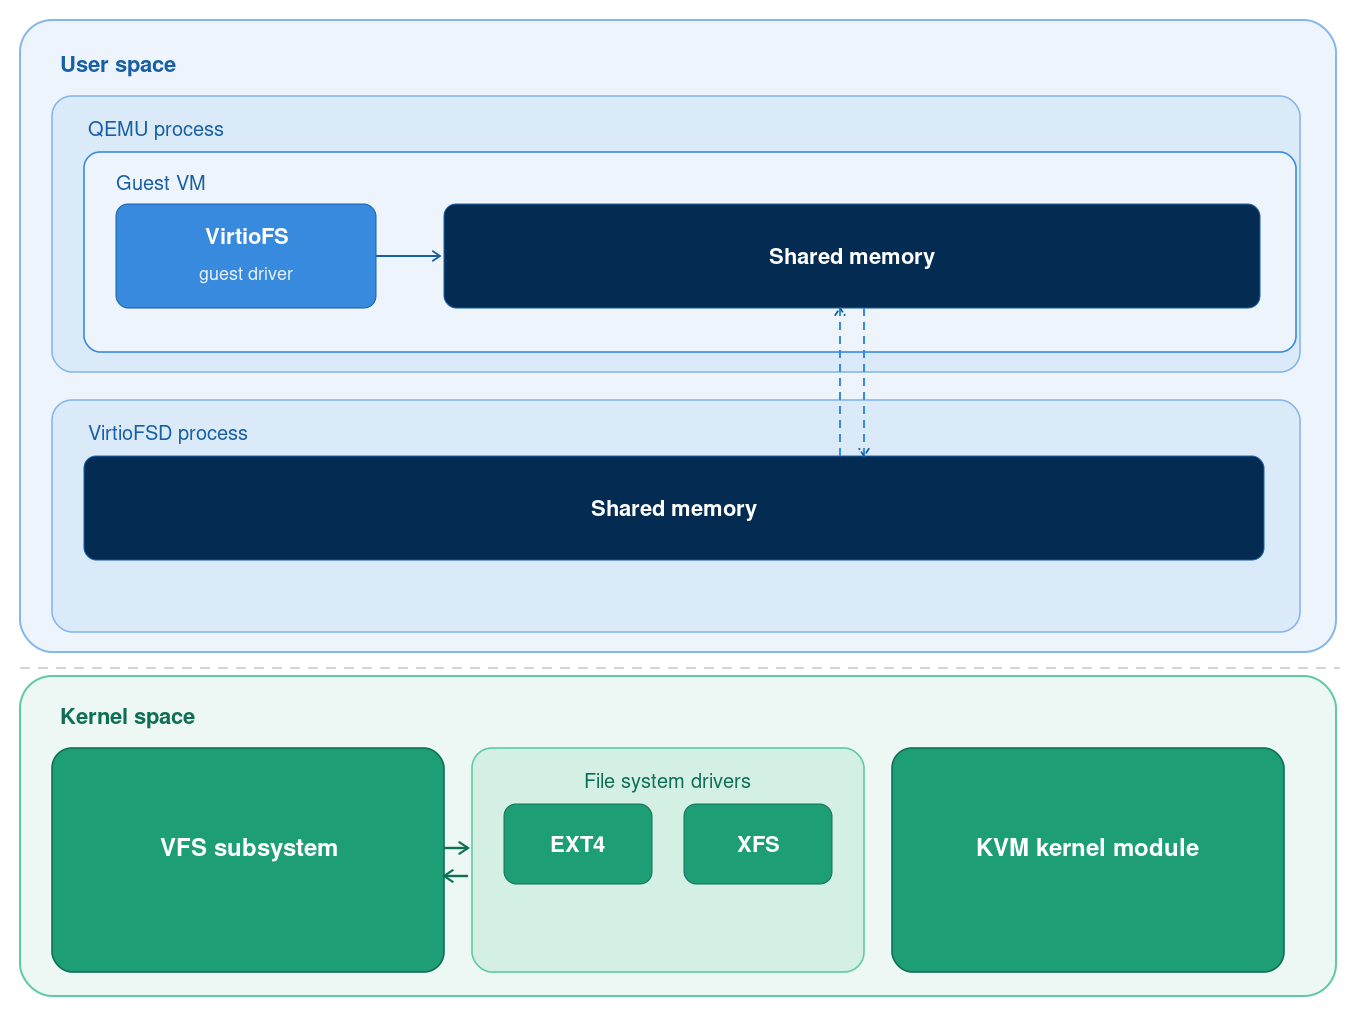
\includegraphics[width=0.90\linewidth]{virtiofs_static.png}
  \caption{VirtioFS static component overview}
  \label{fig:virtiofs_static}
\end{figure}

Queue 0 is the \textit{high-priority} queue for latency-sensitive messages such
as \texttt{FUSE\_FORGET}; queue 1 is the general-purpose \textit{request} queue.
VirtioFS supports scatter-gather I/O: a single descriptor chain may reference
multiple discontiguous guest buffers.

\begin{figure}[htbp]
  \centering
  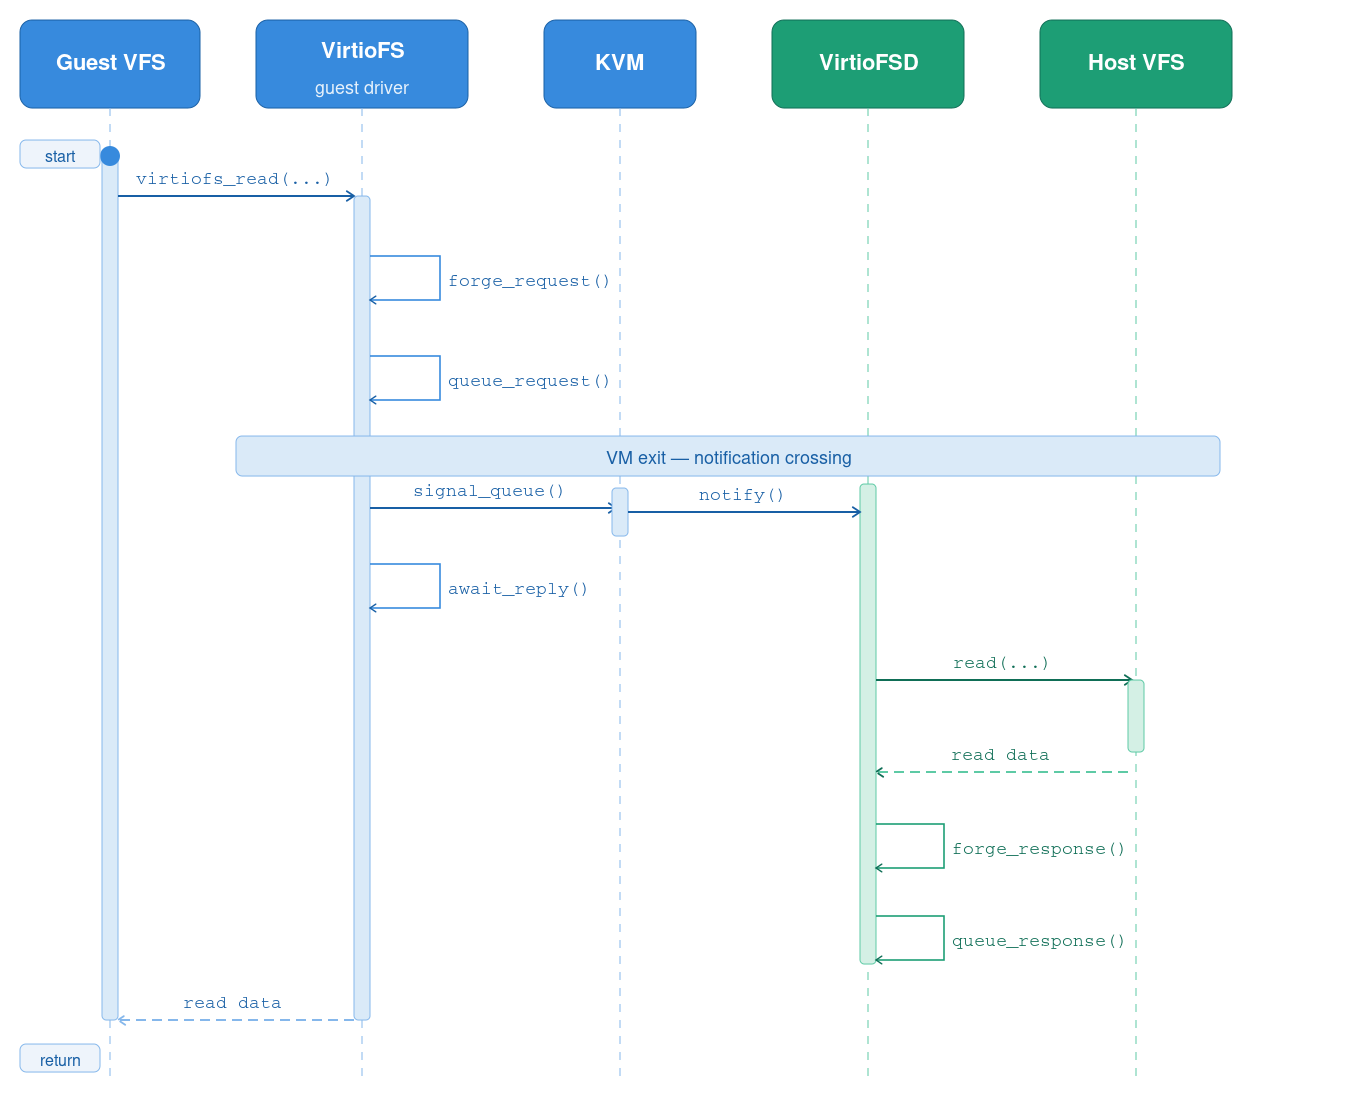
\includegraphics[width=0.80\linewidth]{virtiofs_sequence.png}
  \caption{An abstract sequence diagram modeling a guest read through the VirtioFS stack.
    Blue = guest-side actors; teal = host-side.}
  \label{fig:virtiofs_sequence}
\end{figure}

\section{Dual Ring Buffer}
\label{sec:dualring}

The circular ring buffer is one of the most ubiquitous data structures in
systems programming.  It enables lockless access by having one thread enqueue
entries while another dequeues and consumes them --- as long as only one
producer and one consumer operate concurrently, no locks are required.

The \textbf{dual ring buffer} pattern consists of two circular ring buffers.
The first ring buffer carries requests from client to server; the second carries
responses from server to client.  Together they form a lockless
request--response channel. This abstract pattern is the foundation for both
io\_uring and Virtio. 

\section{Atomics}
Compiler atomics and CPU atomics
% Torn reads and writes
% https://mintomic.github.io/
% x86 loads and stores are atomic

\section{Memory Ordering}
\label{sec:memory}

\subsection{The x86 Memory Model}

The x86 architecture implements a relatively strong memory model known as
\textbf{Total Store Ordering (TSO)}.  Under TSO, read and store instructions
are generally not reordered with one notable exception: older stores may be
reordered with younger loads to \textit{different} memory locations.
Critically, the executing CPU itself still sees a consistent view of its own
memory operations --- the reordering is only visible to \textit{other} CPUs
observing the memory bus.

\subsection{The C++ Memory Model}

The C++ memory model, introduced in C++11, provides a portable abstraction over
hardware memory models.  It defines a set of memory orderings that the programmer
can attach to atomic operations to control visibility and synchronization
guarantees across threads:

In the context of the Virtio split queue, the C++ memory model is applied
precisely: a \texttt{memory\_order\_release} fence is issued after populating
the descriptor chain and before incrementing the available ring index, ensuring
all descriptor writes are visible to the device before it observes the updated
index.  A subsequent \texttt{memory\_order\_seq\_cst} fence precedes the check
of the used ring's notification suppression flag, preventing reordering that
could cause a missed notification.

% https://en.cppreference.com/cpp/atomic/atomic_thread_fence
% Reading the notification flag

% 1. Corrupted virtqueues
% 2. Missing notifications
% Improve usefullness of the ^^^

\section{io\_uring}
\label{sec:iouring}

io\_uring is a modern Linux I/O interface introduced in kernel 5.1, designed to
address the performance inefficiencies of POSIX I/O and earlier asynchronous I/O
mechanisms such as AIO.  The primary selling point of io\_uring is its ability
to greatly reduce --- and in some configurations eliminate entirely --- the
number of system calls required to perform I/O.

io\_uring is built on the dual ring buffer pattern described in
Section~\ref{sec:dualring}.  It exposes two shared-memory ring buffers between
user space and the kernel: the \textbf{submission queue (SQ)}, into which the
application places I/O requests, and the \textbf{completion queue (CQ)}, from
which the application reads completions.  Because both rings live in shared
memory, the application can submit requests and harvest completions without any
system call, provided the kernel is actively polling the submission queue.

io\_uring supports a polling mode called \textbf{SQPOLL}, in which a dedicated
kernel thread continuously polls the submission queue for new entries.  In this
mode, applications can perform I/O with zero system calls for the duration of the
polling window.  When the kernel thread has been idle for a configurable timeout,
it sleeps and requires a wakeup syscall (\texttt{io\_uring\_enter}) to resume.

\textbf{liburing} is a user-space wrapper library around the io\_uring API.
io\_uring's raw interface involves careful management of ring indices, memory
barriers, and kernel flags; liburing encapsulates this complexity and provides a
higher-level interface that substantially reduces the boilerplate required when
writing io\_uring applications.

The architectural similarity between io\_uring and Virtio is not coincidental:
both implement the dual ring buffer pattern over shared memory to decouple
request submission from completion processing, enabling high-throughput
asynchronous I/O without per-operation kernel crossings.

\section{Virtio Standard}
\label{sec:virtio}

\subsection{Introduction}

Virtio~\cite{virtio2024} is a paravirtualization standard for efficient data
exchange between a guest \textit{driver} and a host \textit{device}.  It
separates a \textbf{control plane} --- device discovery, configuration, and
feature negotiation --- from a \textbf{data plane} that exchanges bulk data via
shared-memory ring structures called \textbf{virtqueues}

\subsection{Device Discovery via PCI}

Virtio devices advertise their register regions through vendor-specific PCI
capabilities, each with a \texttt{cfg\_type} identifying the region and
\texttt{bar}, \texttt{offset}, and \texttt{length} fields locating it.  Four
standard Virtio capability types are defined:

\begin{itemize}
  \item \texttt{VIRTIO\_PCI\_CAP\_COMMON\_CFG}: device-wide and per-queue
        configuration registers.
  \item \texttt{VIRTIO\_PCI\_CAP\_NOTIFY\_CFG}: queue notification region.
  \item \texttt{VIRTIO\_PCI\_CAP\_ISR\_CFG}: interrupt status register.
  \item \texttt{VIRTIO\_PCI\_CAP\_DEVICE\_CFG}: device-class-specific registers.
\end{itemize}

The control plane governs the full device lifecycle.  The specification
prescribes strict ordering: reset (\texttt{device\_status = 0}), set
\texttt{ACKNOWLEDGE} and \texttt{DRIVER} bits, negotiate features, set
\texttt{FEATURES\_OK} and verify the device retains it, configure queues, then
set \texttt{DRIVER\_OK}.  After setup, MMIO is used only for queue kicks; under
KVM each kick delivers an \texttt{ioeventfd} notification directly to the device
thread.

\subsubsection{Descriptor Area}

The descriptor area is an array of descriptor entries each carrying a
guest-physical \textbf{Buffer} address, a byte \textbf{Len}, \textbf{Flags}, and a chain
\textbf{Next} index. The \textbf{Next} is valid when the \texttt{NEXT} flag is set in the same entry. A writeable descriptor is distinguished from a readable descriptor by having \texttt{WRITE} flag. Readable descriptors must precede all writable descriptors --- no interleaving is permitted.

\subsubsection{Available and Used Areas}

The driver and device communicate using two areas with similar structure: Available and used area. The areas \textbf{MUST} only be modified by one end and read by the other. The driver modifies the available area while the device modifies the used area. The driver reads the used area while the device reads the available area. The areas follow the dual ring buffer pattern described in section~\ref{sec:dualring} with additional flag fields for signaling that notifications are not needed for processing the request.

\subsubsection{Request Submission --- Driver to Device}

The driver allocates free descriptors, populates them, links them via the
\texttt{next} field, places the head index into the available ring's
\texttt{ring[]}, and increments the available ring's \texttt{idx} to expose the
request.  A \texttt{memory\_order\_release} fence precedes the counter advance.
The driver then conditionally writes the queue index to the notification register
to kick the device. The tracks request by comparing \texttt{\_avail\_ring->idx} against its locally maintained \texttt{\_last\_avail\_idx}. 

\begin{figure}[htbp]
  \centering
  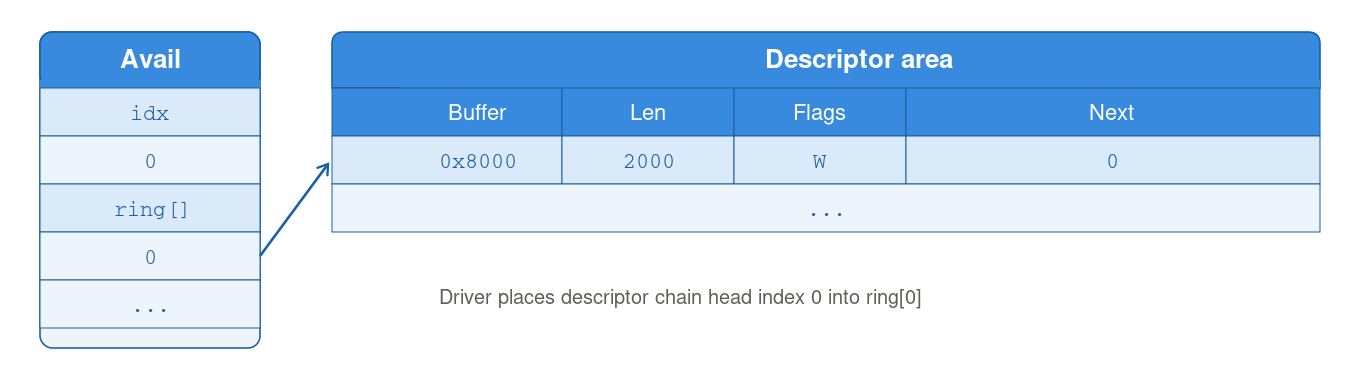
\includegraphics[width=0.85\linewidth]{avail_enqueue.png}
  \caption{Driver places descriptor chain head index 0 into \texttt{ring[0]}.}
  \label{fig:avail_enqueue}
\end{figure}

\begin{figure}[htbp]
  \centering
  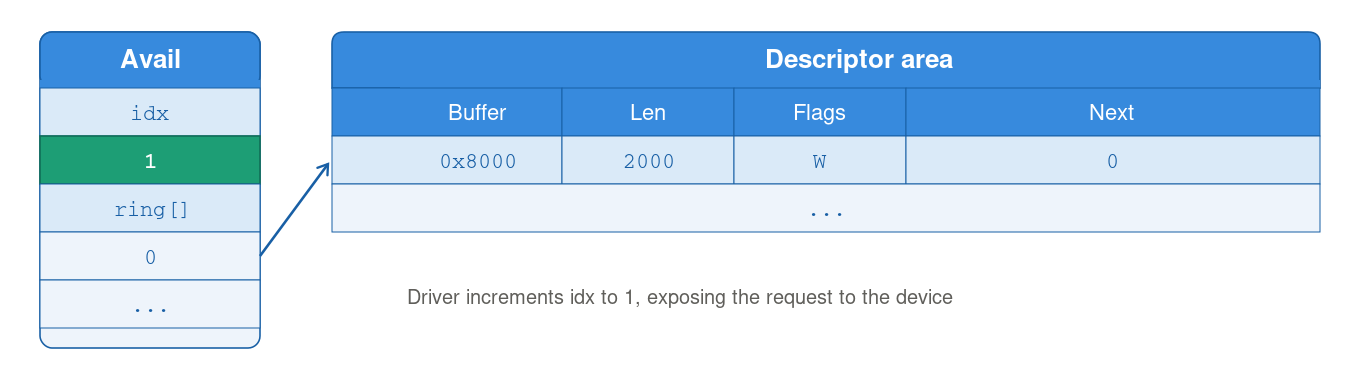
\includegraphics[width=0.85\linewidth]{avail_expose.png}
  \caption{Driver increments \texttt{idx} to 1 (green), exposing the request.}
  \label{fig:avail_expose}
\end{figure}

\subsubsection{Request Completion --- Device to Driver}

After processing a request, the device writes a \texttt{virtq\_used\_elem} ---
containing the head descriptor index and bytes written into writable buffers ---
and increments the used ring's \texttt{idx}. A store fence \textbf{MUST} precede the increment \ref{sec:memory}. The driver detects completion by
comparing \texttt{\_used\_ring->idx} against its locally maintained
\texttt{last\_used\_idx}.

\begin{figure}[htbp]
  \centering
  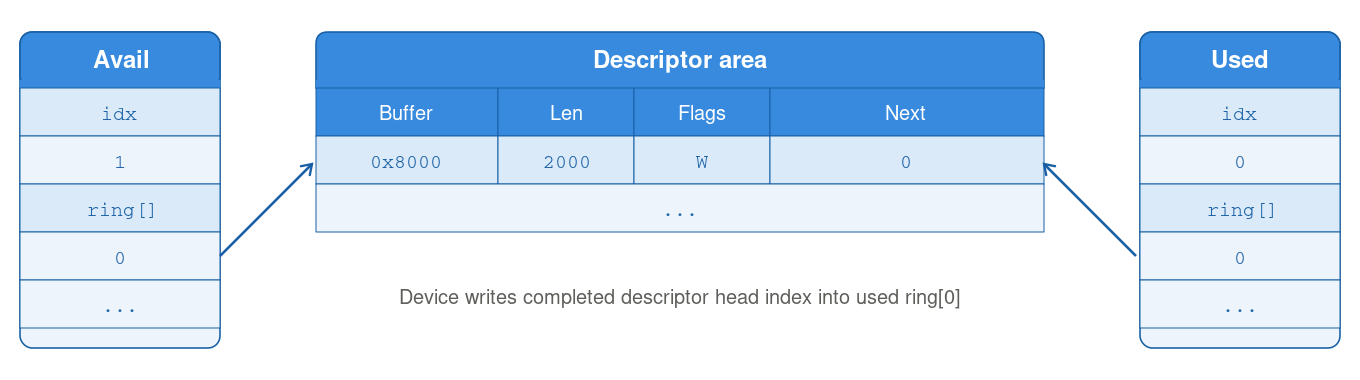
\includegraphics[width=0.85\linewidth]{used_enqueue.png}
  \caption{Device writes the completed descriptor head index into used
           \texttt{ring[0]}.}
  \label{fig:used_enqueue}
\end{figure}

\begin{figure}[htbp]
  \centering
  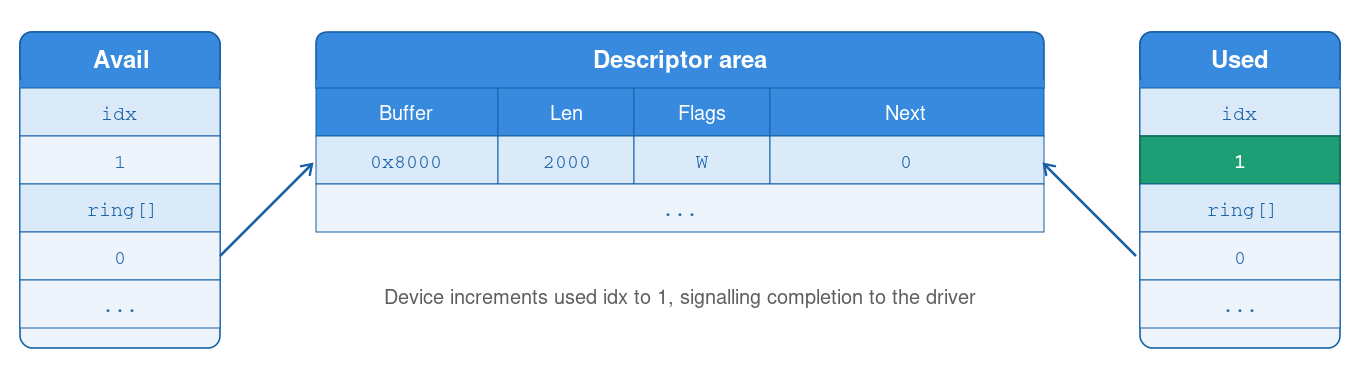
\includegraphics[width=0.85\linewidth]{used_expose.png}
  \caption{Device increments used \texttt{idx} to 1 (green), signalling
           completion.}
  \label{fig:used_expose}
\end{figure}

\begin{figure}[htbp]
  \centering
  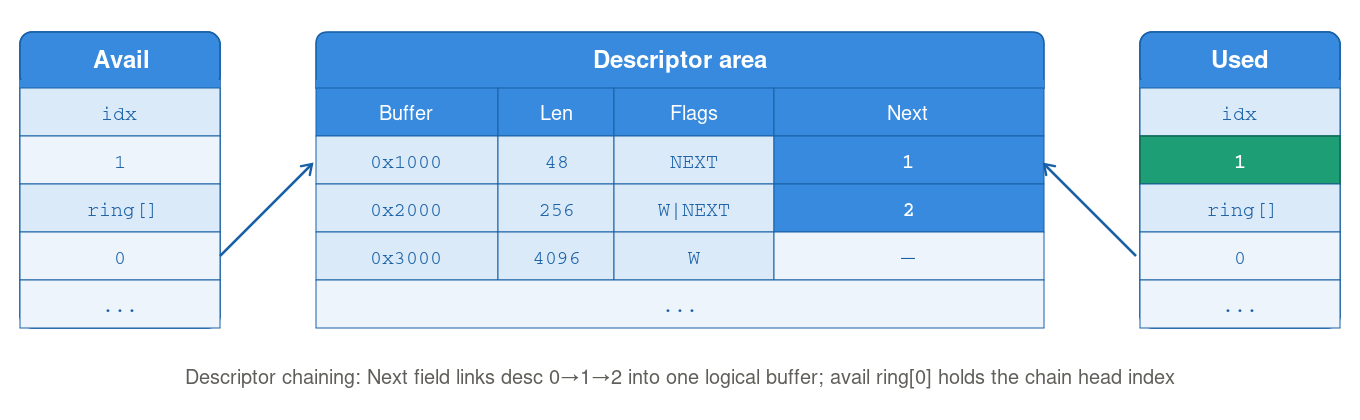
\includegraphics[width=0.85\linewidth]{desc_chain.png}
  \caption{Descriptor chaining: the \texttt{Next} field of descriptor~0
           (head, placed in \texttt{avail.ring[0]}) points to descriptor~1,
           which in turn points to descriptor~2 (end of chain, no
           \texttt{NEXT} flag).  The device processes all three as a single
           logical scatter-gather buffer; the used ring returns the head
           index~0 on completion.}
  \label{fig:desc_chain}
\end{figure}

\subsubsection{Notification Mechanisms}

Both sides can suppress notifications.  The driver sets
\texttt{VIRTQ\_AVAIL\_F\_NO\_INTERRUPT} to inhibit device interrupts; the device
sets \texttt{VIRTQ\_USED\_F\_NO\_NOTIFY} to inhibit driver kicks.  These flags
enable runtime switching between interrupt-driven and polling modes.

\subsection{Fences are complicated}
% Missing notifications
% Virtqueue corruption
% Reference code on my github profile
% Reference git commit patches

\section{FUSE}
\label{sec:fuse}

\subsection{Protocol}

FUSE~\cite{fuse2024} exports file-system operations to a user-space server.
Every request begins with \texttt{fuse\_in\_header} carrying the opcode, total
length, a monotonically increasing \texttt{unique} identifier, and the target
inode number.  Every response begins with \texttt{fuse\_out\_header} echoing
\texttt{unique} and an error code.

\subsection{Initialization Handshake}

Client and server negotiate protocol version via \texttt{FUSE\_INIT}.  The
client advertises its major and minor versions; the negotiated minor is the
minimum of the two.  If the server's major is lower, the client must re-send
adjusted to the server's major.  The response carries \texttt{max\_write} ---
the maximum payload the server accepts per write.  The client must cache and
enforce this limit.

\subsection{File Operations}

A complete read sequence issues: \texttt{FUSE\_LOOKUP} (path $\to$ inode),
\texttt{FUSE\_OPEN} (inode $\to$ 64-bit file handle), \texttt{FUSE\_READ}
(file handle, buffer, offset, length), \texttt{FUSE\_RELEASE} (free file
handle), and \texttt{FUSE\_FORGET} (decrement inode reference count).  Writes
follow an analogous pattern; \texttt{FUSE\_CREATE} combines lookup and open for
new files.

\section{IncludeOS}
\label{sec:includeos}

\subsection{Overview}

IncludeOS~\cite{bratterud2015} is a lightweight, bootable operating system
implemented in C, C++, and assembly.  Unlike conventional operating systems,
IncludeOS follows the \textbf{unikernel} paradigm: it packages an application
together with only the essential libraries and device drivers required for
execution.  The result is a single-address-space image with no process isolation,
no user/kernel boundary, and no general-purpose scheduler.  This design enables
substantial reductions in both CPU and memory consumption compared to traditional
virtual machines.  The virtual address space is configured with identity mapping
to physical memory for the first 512~GiB.

\subsection{PCI Interface}

Driver implementations receive a reference to a generic PCI device abstraction
during construction.  This abstraction exposes methods for PCI configuration
space access (\texttt{read16}, \texttt{read32}), capability discovery
(\texttt{probe\_resources}, \texttt{parse\_capabilities}), and MSI-X management
(\texttt{msix\_cap}, \texttt{init\_msix}, \texttt{get\_msix\_vectors}).  Before
utilizing MSI-X functionality, drivers must invoke \texttt{probe\_resources()}
and \texttt{parse\_capabilities()} to enumerate available resources.  Following
these preparatory calls, \texttt{init\_msix()} configures MSI-X support, and
\texttt{get\_msix\_vectors()} returns the number of available interrupt vectors.
MSI-X vector identifiers are valid in the range zero to vector count exclusive.

% Shit, improve by adding some kind of class diagram?
% Backlink to this

\subsection{Events and Interrupts}
\label{sec:includeos_events_irqs}

IncludeOS implements interrupt handling through an event-driven architecture
based on callback queues.  When a hardware interrupt fires, the system executes
the delegate registered for the corresponding event number.  A driver registers
a delegate with \texttt{Events::get().subscribe()}, receiving an event number.
This event number is then configured as the target for a specific interrupt
vector via \texttt{setup\_msix\_vector()}.  When the configured interrupt fires,
the registered delegate executes asynchronously.

\begin{figure}[htbp]
  \centering
  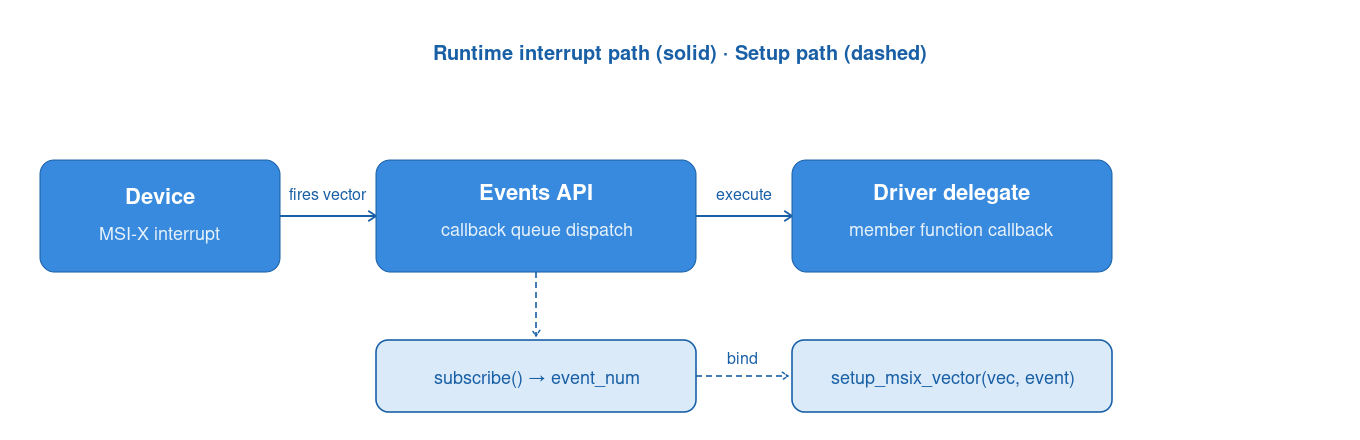
\includegraphics[width=0.88\linewidth]{includeos_interrupt.png}
  \caption{IncludeOS interrupt handling.  Setup path (dashed): the driver
    subscribes a delegate to get an event number, then binds it to an MSI-X
    vector.  Runtime path (solid): the device fires the vector, the Events
    API dispatches to the registered delegate.}
  \label{fig:includeos_interrupt}
\end{figure}

\subsection{Filesystem Support and MUSL Integration}

IncludeOS provides filesystem functionality through two complementary approaches:
a POSIX-compatible interface via the MUSL C standard library~\cite{musl2024}, and
native IncludeOS filesystem abstractions.  The filesystem implementation includes
standard file descriptor abstractions for both generic and filesystem-specific
descriptors.  Filesystem paths are represented as tokenized strings using the
forward slash as a separator.

IncludeOS integrates MUSL, a minimal implementation of the C standard library
widely adopted in embedded systems development, distinguished by its low memory
overhead.  IncludeOS employs a patched version of MUSL that redirects standard
system calls to external functions, enabling customization of system call
behaviour.  This patching mechanism, implemented in
\texttt{src/musl/*.cpp}, allows IncludeOS to intercept and reimplement standard
library system calls to align with the unikernel execution model --- making it
possible for applications to use VirtioFS transparently through standard POSIX
file I/O without any application-level awareness of the underlying Virtio
transport.

% ════════════════════════════════════════════════════════════════════════════
%  CHAPTER 3 — DESIGN
% ════════════════════════════════════════════════════════════════════════════
\chapter{Design}
\label{chap:design}

The VirtioFS driver is structured as three cooperating layers: a virtual
filesystem (VFS) abstraction layer interfacing with the POSIX system-call layer;
a Virtio PCI transport layer managing device initialization and queue operations;
and a VirtioFS device layer composing the two lower layers into a complete
VirtioFS.

\section{Virtual Filesystem Layer}
\label{sec:design-vfs}

The VFS layer is deliberately thin: it performs path-based dispatch and
file-descriptor bookkeeping, delegating all actual I/O to the registered driver.
Four cooperating components form the layer:

\begin{itemize}
  \item \texttt{fs::VFS} --- singleton mount table mapping string prefixes to
        \texttt{fs::Filesystem} structs of function pointers (\texttt{open},
        \texttt{read}, \texttt{readv}, \texttt{write}, \texttt{writev},
        \texttt{lseek}, \texttt{close}, \texttt{unlink}).
  \item \texttt{FD\_map} --- file-descriptor allocator issuing integer
        descriptors mapped to polymorphic \texttt{FD} objects.
  \item \texttt{File\_FD} --- concrete file descriptor forwarding each method
        call with the descriptor integer to the owning driver's function pointer.
  \item Syscall stubs --- outermost layer performing only path decomposition,
        returning standard \texttt{errno} values on failure.
\end{itemize}

A path such as \texttt{VirtioFS0/data/file.txt} is split at the first separator:
the leading component selects the driver; the tail is forwarded.  Writes to
descriptors 1 and 2 are intercepted before any \texttt{FD\_map} lookup and
routed to \texttt{os::print}.

\section{Virtio PCI Layer}
\label{sec:design-virtio}

The Virtio PCI layer is divided into two independent components reflecting the
specification's separation of control-plane initialization and data-plane I/O.
Keeping them separate allows the future implementation queue implementations such as packed queues.

\texttt{Virtio\_control} encapsulates the full initialization sequence ---
device validation, capability discovery, reset, status-bit sequencing, and
feature negotiation --- completing before returning.  Any failure triggers
\texttt{\_virtio\_panic}, setting \texttt{VIRTIO\_CONFIG\_S\_FAILED} and halting
via \texttt{os::panic}.  \texttt{VIRTIO\_F\_VERSION\_1} is unconditionally
required; optional features are accepted only if the device advertises them.

Virtio\_control required and optional features are passed by the constructor down to the \_negotiate\_features (called by the constructor) method. Virtio\_control an optional method for enabling MSI-X interrupts for deferred queue callback routines. Add a flowchart here!

Virtio\_control exposes that is required by every device to call for finishing the Virtio PCI plane initialization sequence. That function is called set\_driver\_ok\_bit. This function is called after the Virtio\_control constructor, virtqueue constructors. Afterwards, the virtqueues are functional and operating. 

% Class diagram may be useful here!

\texttt{Split\_queue} implements the split virtqueue, exposing direct control
over descriptor chain composition for arbitrary scatter-gather I/O patterns.  At
construction it validates \texttt{queue\_size}, allocates the three ring
structures with mandated alignments, registers their physical addresses, and
computes the per-queue notification address.  A free-descriptor pool provides
O(1) allocation and reclamation with no dynamic memory allocation on the I/O
path.

\section{VirtioFS Device}
\label{sec:design-device}

The VirtioFS device driver composes one \texttt{Virtio\_control} and two
\texttt{Split\_queue} instances into a POSIX filesystem interface.  Queue 0 is
the high-priority queue; queue 1 the request queue.  Both are configured in
polling mode (\texttt{VIRTIO\_MSI\_NO\_VECTOR}).

% The different versions use 

\subsection{Initialization Sequence}

\begin{figure}[htbp]
  \centering
  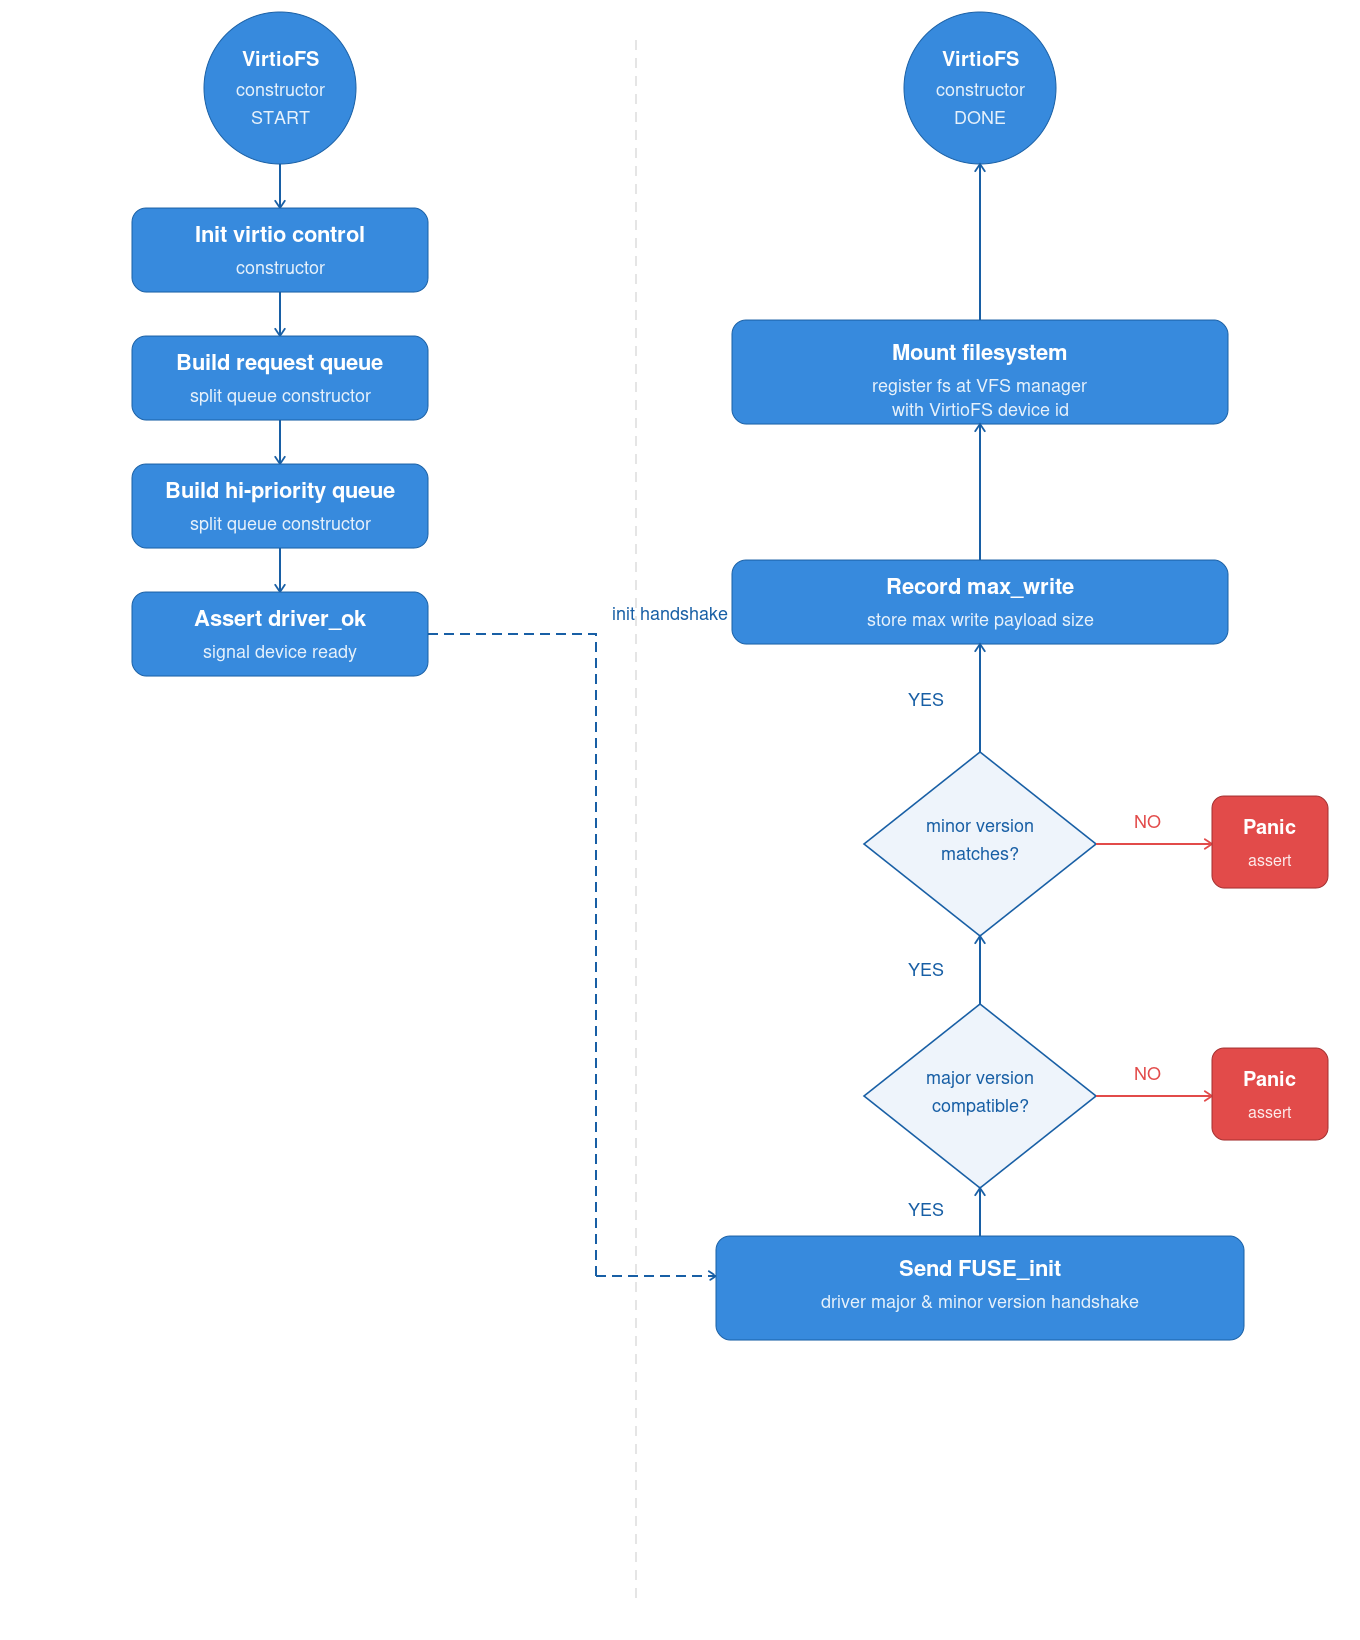
\includegraphics[width=0.76\linewidth]{virtiofs_init.png}
  \caption{VirtioFS constructor initialization sequence.  Left (top-down):
    Virtio setup.  Right (bottom-up): FUSE handshake, version checks,
    \texttt{max\_write} record, filesystem mount.}
  \label{fig:virtiofs_init}
\end{figure}

Initialization proceeds in three sequential phases.  First,
\texttt{Virtio\_control} completes PCI negotiation, both queues are registered,
and \texttt{set\_driver\_ok\_bit} signals readiness.  Second, the
\texttt{FUSE\_INIT} handshake advertises major version 7 and minor version 36;
version numbers are validated and \texttt{max\_write} is stored, reduced by
\texttt{FUSE\_BUFFER\_HEADER\_SIZE}.  Third, an \texttt{fs::Filesystem} struct
is registered with \texttt{fs::VFS} under \texttt{VirtioFS\{id\}}.

% I need to talk about MAX_WRITE

\subsection{Synchronous Polling Model}

All filesystem operations are \textit{synchronous and blocking}: at most one
request is in flight at any time, and the CPU spins on
\texttt{has\_processed\_used} until completion.  Busy-waiting in this manner
eliminates scheduling latency and maximizes I/O throughput.  Request
headers are allocated on the stack; caller-supplied buffers are enqueued directly as
Virtio descriptor tokens, delivering data between caller memory and VirtioFSD
without any intermediate copies.

\subsection{Combined Interaction}

Figure~\ref{fig:virtio_pci_sequence} shows the full lifetime of the three
cooperating components across initialization and a single I/O operation.

\begin{figure}[htbp]
  \centering
  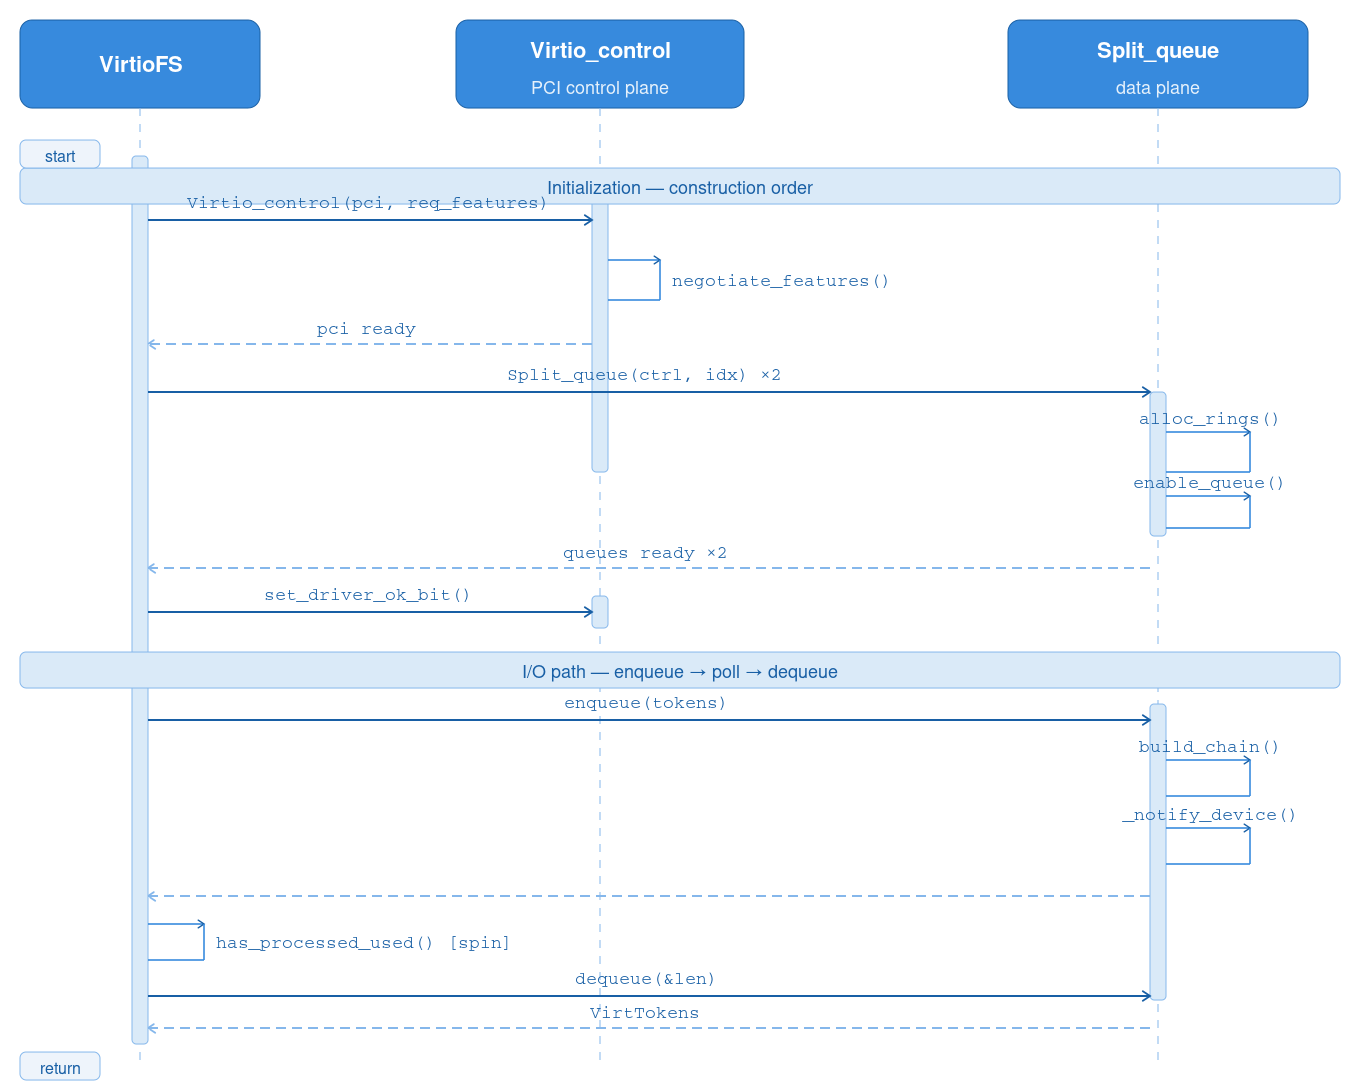
\includegraphics[width=0.90\linewidth]{virtio_pci_sequence.png}
  \caption{Sequence diagram of the combined interaction between
    \texttt{VirtioFS}, \texttt{Virtio\_control}, and \texttt{Split\_queue}.
    The initialization phase (top) establishes the Virtio PCI control plane and
    activates both queues before signalling driver readiness.
    The I/O path (bottom) shows a single request cycle: descriptor chain
    assembly, device notification, synchronous busy-wait, and dequeue.}
  \label{fig:virtio_pci_sequence}
\end{figure}

During initialization \texttt{VirtioFS} first constructs \texttt{Virtio\_control},
which drives the full PCI negotiation sequence --- reset, feature negotiation,
and \texttt{FEATURES\_OK} --- before returning.  Both \texttt{Split\_queue}
instances are then constructed, each selecting its queue slot, allocating the
three ring structures with mandated alignments, registering their physical
addresses, and enabling the queue.  A final call to \texttt{set\_driver\_ok\_bit}
signals device readiness and concludes the control-plane setup.

On the I/O path, \texttt{VirtioFS} calls \texttt{enqueue} on the appropriate
\texttt{Split\_queue} with a \texttt{VirtTokens} vector.  \texttt{Split\_queue}
builds the descriptor chain, issues a release fence to guarantee descriptor
visibility, increments the available ring index, and calls
\texttt{\_notify\_device} to write the queue index to the pre-computed
notification register address.  \texttt{VirtioFS} then busy-waits on
\texttt{has\_processed\_used} until the device writes a completion entry into
the used ring, after which \texttt{dequeue} reclaims the descriptors and returns
the \texttt{VirtTokens} to the caller.

Figure~\ref{fig:virtio_pci_sequence_irq} shows the same lifecycle with MSI-X
interrupts substituted for busy-polling.  The initialization phase extends with
three additional steps: \texttt{enable\_msix} configures the PCI MSI-X capability
and returns the available vector count; \texttt{Events::subscribe} registers a
completion callback in the IncludeOS event system and returns an event number;
and \texttt{setup\_msix\_vector} binds that interrupt vector to the request
queue.  On the I/O path the spin loop is replaced by a \texttt{HLT} instruction
that suspends the vCPU until the device fires a MSI-X interrupt, which the
hypervisor delivers as a virtual interrupt and IncludeOS dispatches to the
registered callback.  Interrupt-driven completion frees the virtual processor for
other work at the cost of additional context-switch latency compared with the
polling model.

\begin{figure}[htbp]
  \centering
  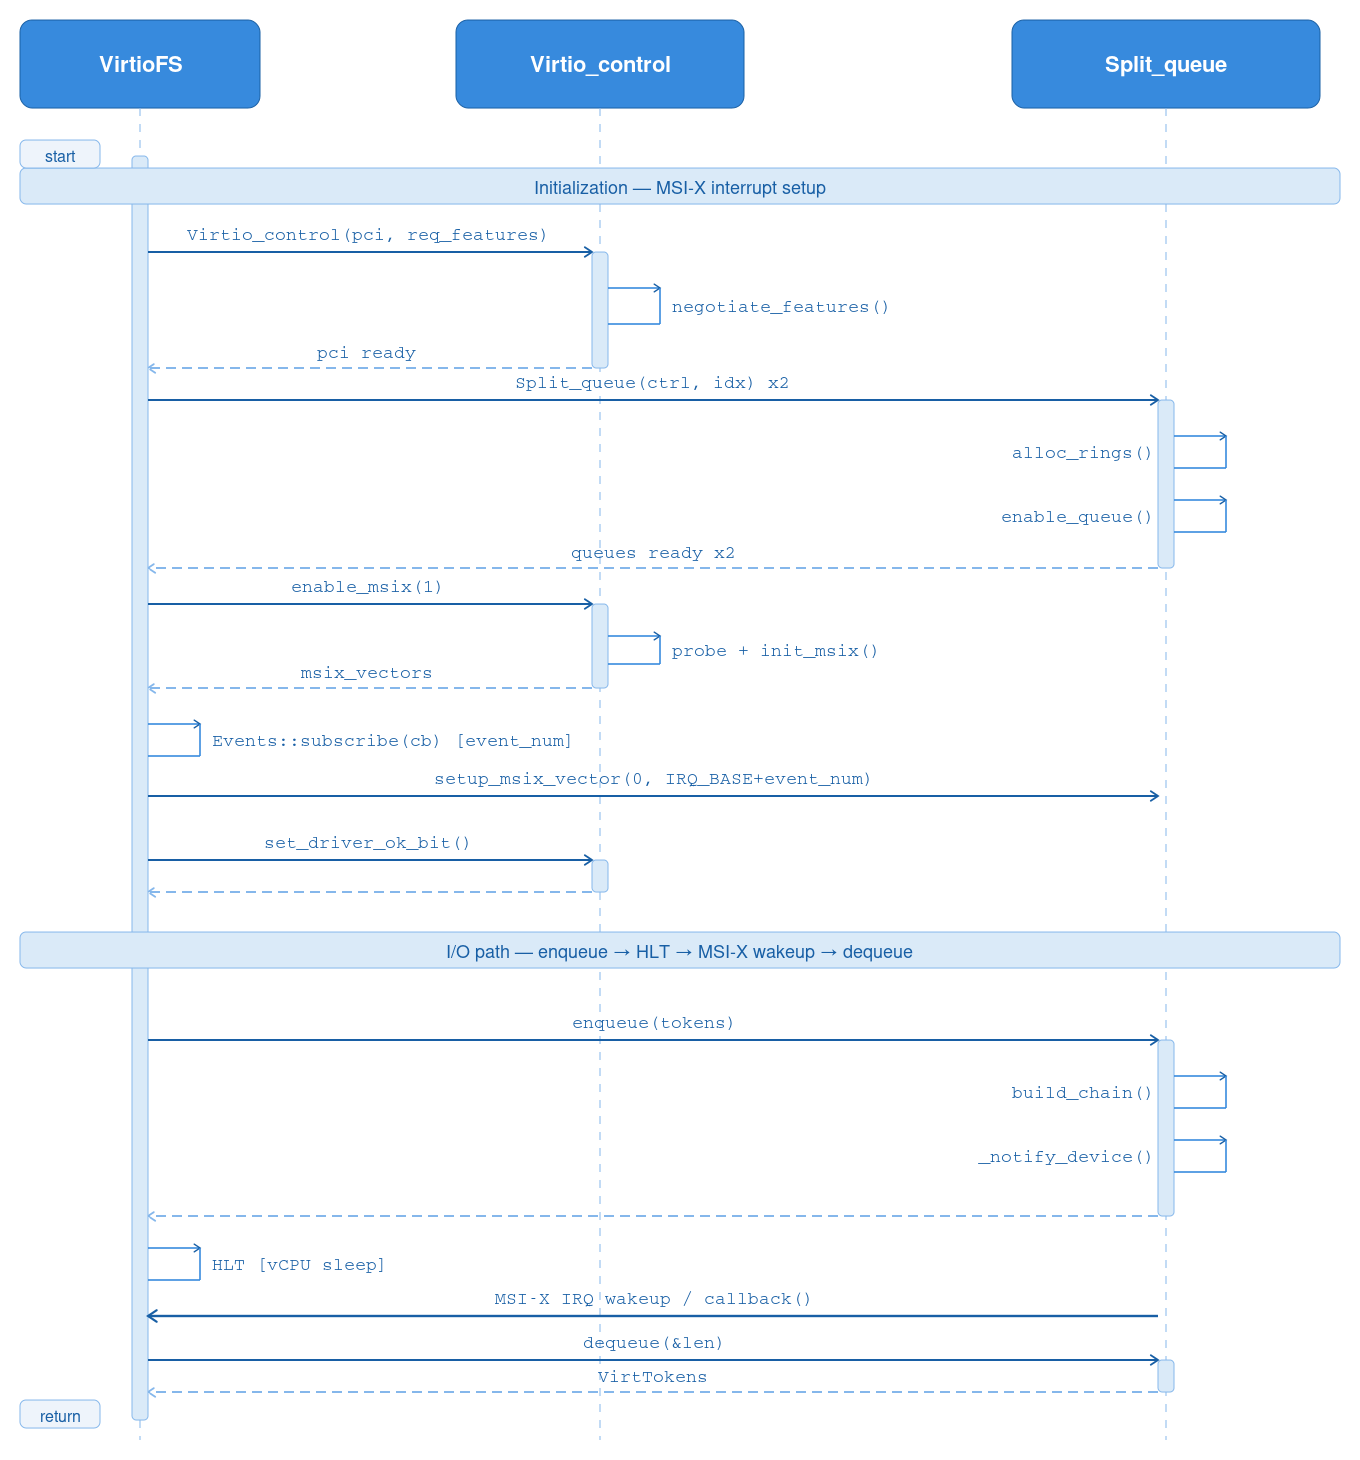
\includegraphics[width=0.90\linewidth]{virtio_pci_sequence_irq.png}
  \caption{Sequence diagram of the interrupt-driven (MSI-X) variant.
    Compared with Figure~\ref{fig:virtio_pci_sequence}, the initialization phase
    adds \texttt{enable\_msix}, \texttt{Events::subscribe}, and
    \texttt{setup\_msix\_vector} calls; the busy-poll spin is replaced by a
    \texttt{HLT} sleep and a \texttt{MSI-X IRQ} wakeup arrow from the device.}
  \label{fig:virtio_pci_sequence_irq}
\end{figure}

% ════════════════════════════════════════════════════════════════════════════
%  CHAPTER 4 — IMPLEMENTATION
% ════════════════════════════════════════════════════════════════════════════
\chapter{Implementation}
\label{chap:implementation}

\section{Virtual Filesystem Layer}
\label{sec:impl-vfs}

The VFS layer sits between the MUSL system call stubs and the registered
filesystem driver.  It is responsible for exactly two concerns: path-based mount
dispatch during \texttt{open}, and file-descriptor-based dispatch for all
subsequent I/O.  Four syscall groups emerge from the implementation, each with a
clearly defined pattern.

\subsection{sys\_open}

\texttt{sys\_open} is the only syscall that touches the mount table.  The raw
pathname is parsed into an \texttt{fs::Path} object, which tokenizes the string
on the forward slash separator.  The leading component --- the mount prefix ---
is extracted via \texttt{path.front()} and looked up in
\texttt{fs::VFS::get\_mounts()}.  If no matching mount exists,
\texttt{-ENOENT} is returned immediately.

If the prefix resolves, the tail path is reconstructed via
\texttt{path.pop\_front()} and \texttt{path.to\_string()} with a trailing
separator stripped.  A \texttt{File\_FD} object is then allocated from
\texttt{FD\_map::\_open<File\_FD>(fs)}, which binds the file descriptor to the
resolved \texttt{fs::Filesystem} struct at allocation time --- this binding is
the key structural decision: all subsequent I/O on this descriptor will dispatch
through the function pointer table captured here, with no further mount table
involvement.  The integer descriptor is retrieved via \texttt{fde.get\_id()} and
passed --- along with the tail path, flags, and mode --- to the driver's
\texttt{open} function pointer.

On success (result == 0) the integer descriptor is returned to the caller.  On
any failure the descriptor must be explicitly released via
\texttt{FD\_map::close(fd)} to avoid leaking it.  The catch block distinguishes
two failure modes by inspecting whether \texttt{fd} is still zero: if so, the
\texttt{FD\_map} allocation itself failed (\texttt{-ENOENT}); otherwise the
driver's open function threw (\texttt{-ENOSYS}).

\begin{figure}[htbp]
  \centering
  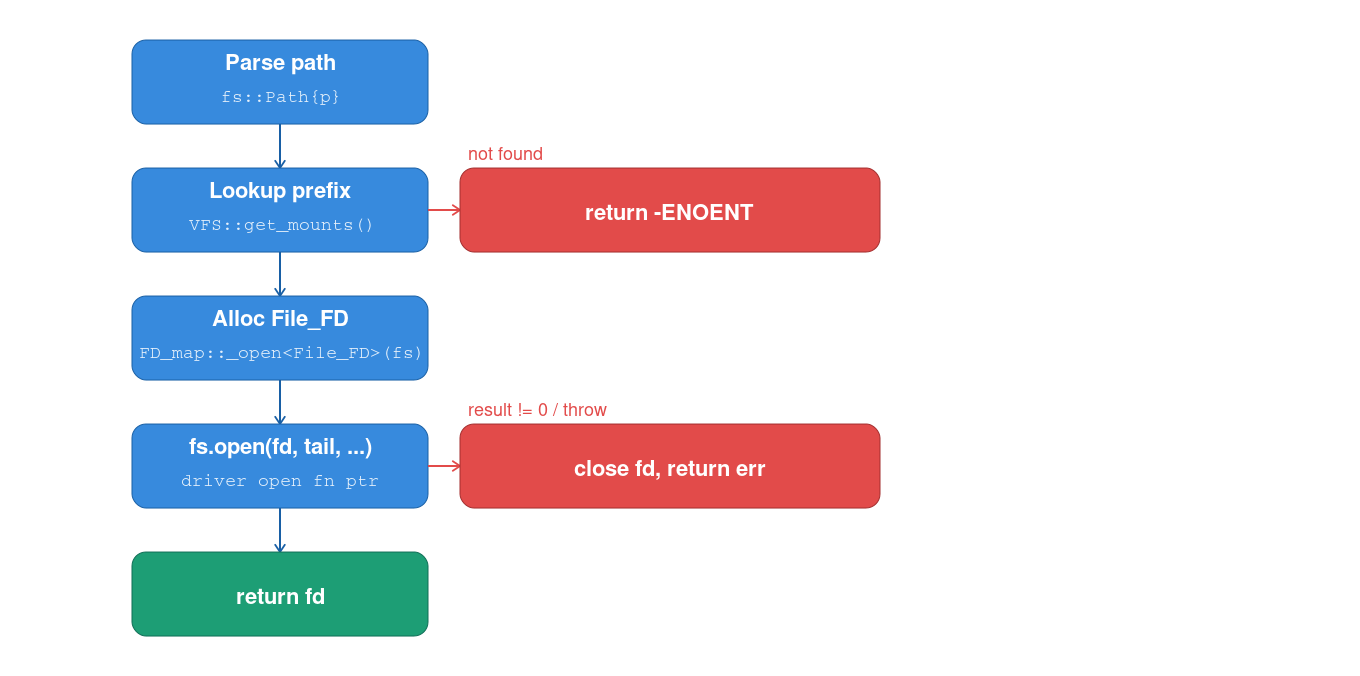
\includegraphics[width=0.90\linewidth]{vfs_sys_open.png}
  \caption{\texttt{sys\_open}: path parse, prefix lookup, \texttt{File\_FD}
           allocation, and driver call.}
  \label{fig:vfs_sys_open}
\end{figure}

\subsection{sys\_read / sys\_readv / sys\_write / sys\_writev}

These four syscalls share a common structural pattern.  Each follows the same
three-step skeleton: call \texttt{FD\_map::\_get(fd)} to retrieve the
\texttt{File\_FD*} associated with the integer descriptor; if non-null, invoke
the corresponding virtual method on the \texttt{File\_FD}, which forwards
through the \texttt{fs::Filesystem} function pointer to the driver; return
\texttt{-EBADF} if the pointer is null or \texttt{-ENOSYS} if the driver throws.
The VFS layer itself contains no I/O logic --- all behaviour is entirely
delegated.

\texttt{sys\_write} and \texttt{sys\_writev} diverge from this pattern for file
descriptors 1 (stdout) and 2 (stderr).  Both check for these reserved values
\textit{before} any \texttt{FD\_map::\_get} call and route output directly to
\texttt{os::print()}, bypassing the VFS entirely.  For \texttt{sys\_writev},
each \texttt{iovec} element is printed individually in a loop.  This intercept
allows the C standard library output functions to work before any filesystem
driver is registered, and without driver dispatch overhead.

\begin{figure}[htbp]
  \centering
  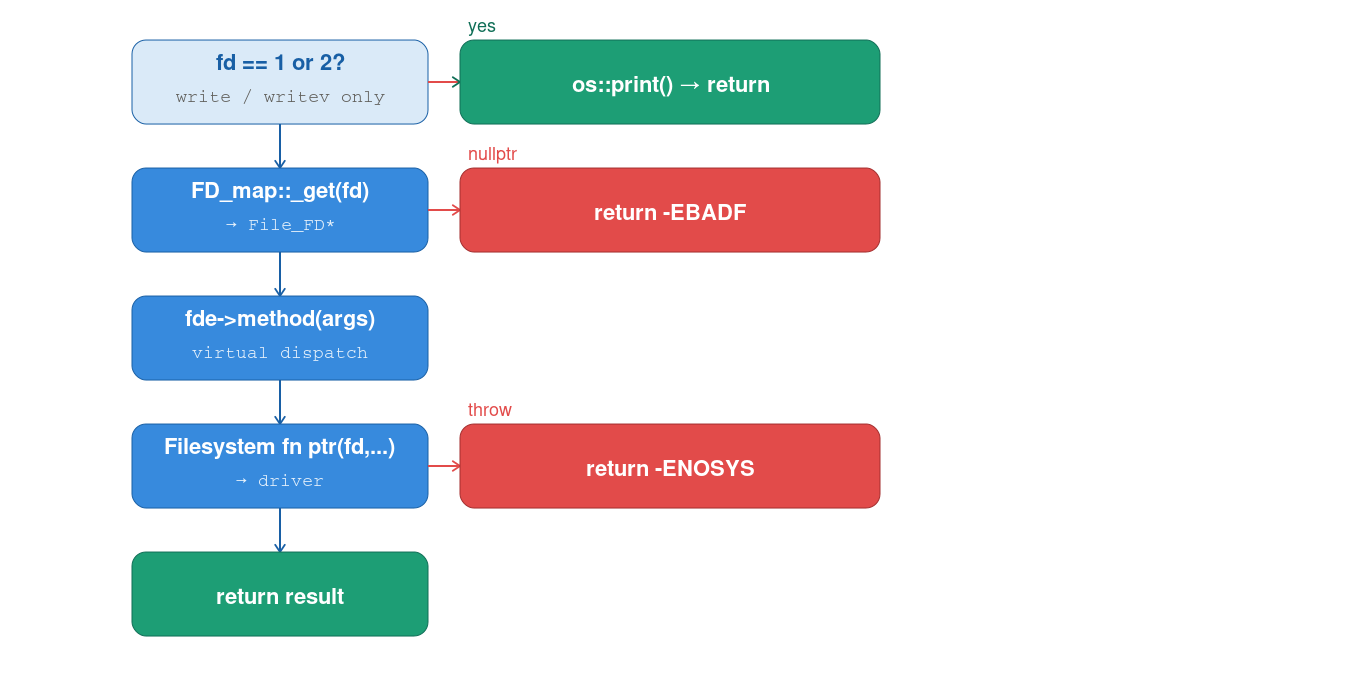
\includegraphics[width=0.90\linewidth]{vfs_sys_io.png}
  \caption{\texttt{sys\_read}/\texttt{readv}/\texttt{write}/\texttt{writev}:
           stdout/stderr intercept (write/writev only), then shared fd dispatch
           through \texttt{FD\_map}, virtual method, and driver function pointer.}
  \label{fig:vfs_sys_io}
\end{figure}

\subsection{sys\_close}

\texttt{sys\_close} follows the same \texttt{FD\_map::\_get} lookup as the I/O
group, but diverges in two important ways.  First, it checks explicitly for a
null \texttt{File\_FD*} and returns \texttt{-EBADF} rather than relying on the
try-catch path.  Second, a non-zero return from the driver's \texttt{close}
method is treated as unrecoverable: \texttt{sys\_close} calls
\texttt{os::panic()} with a diagnostic message rather than propagating the error
upward.  The fd is released via \texttt{FD\_map::close(fd)} only after a
successful driver close --- ensuring the descriptor is not reissued while the
driver still holds resources associated with it.

\begin{figure}[htbp]
  \centering
  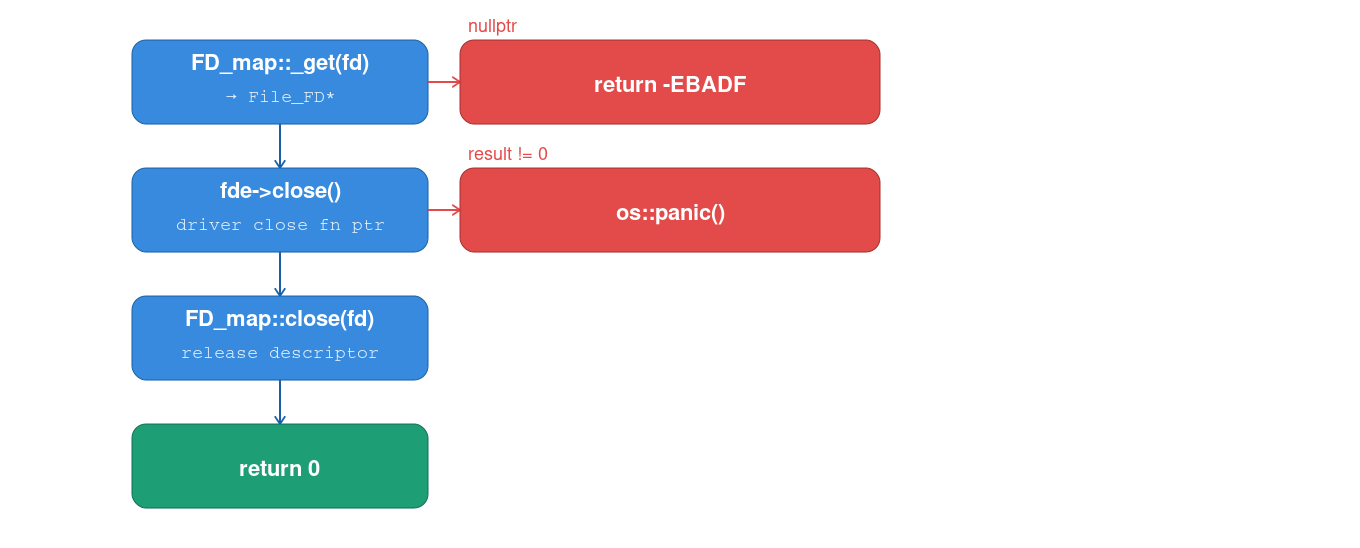
\includegraphics[width=0.90\linewidth]{vfs_sys_close.png}
  \caption{\texttt{sys\_close}: explicit null check, driver close with panic on
           failure, then descriptor release.}
  \label{fig:vfs_sys_close}
\end{figure}

\subsection{sys\_unlink}

\texttt{sys\_unlink} follows the same prefix-extraction pattern as
\texttt{sys\_open} --- parse, \texttt{front()}, \texttt{contains()},
\texttt{pop\_front()}, \texttt{to\_string()}, strip --- but skips fd allocation
entirely and calls the driver's \texttt{unlink} function pointer directly with
the tail path.  It uses a \texttt{submount\_exists} boolean flag to distinguish
between a missing mount (\texttt{-ENOSYS}) and a driver-thrown error
(\texttt{-ENOENT}) in the catch block.  \texttt{sys\_unlink} is therefore the
simplest syscall in the group: no fd lifecycle, no stdout intercept, just mount
resolution and a direct driver call.

\begin{figure}[htbp]
  \centering
  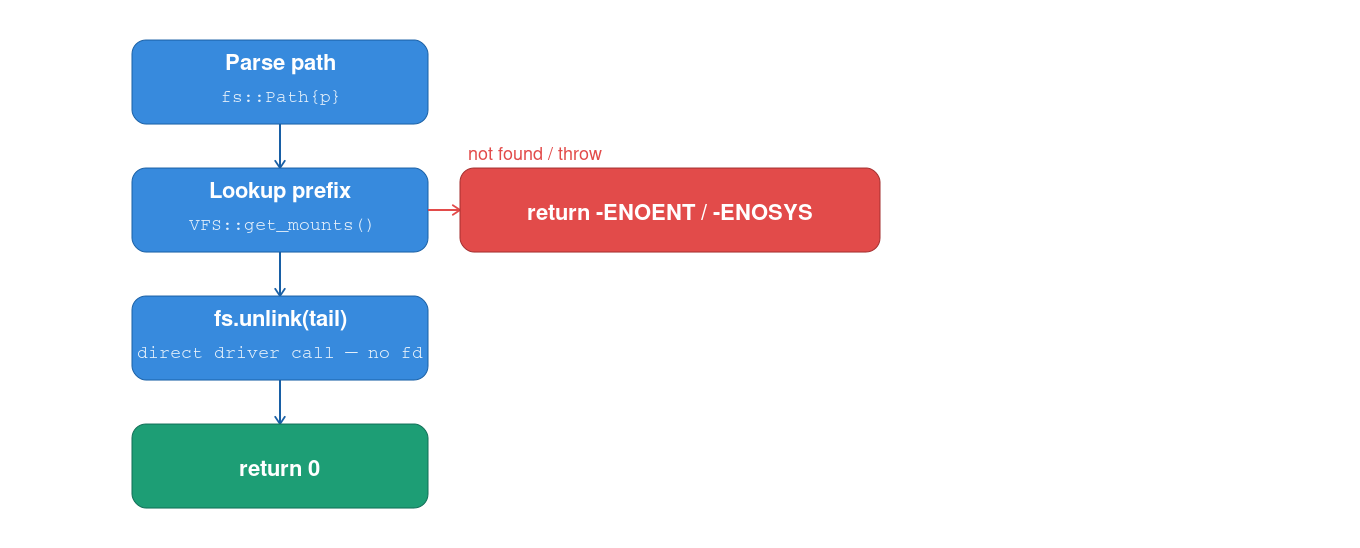
\includegraphics[width=0.90\linewidth]{vfs_sys_unlink.png}
  \caption{\texttt{sys\_unlink}: same prefix lookup as \texttt{sys\_open},
           direct driver call, no fd lifecycle.}
  \label{fig:vfs_sys_unlink}
\end{figure}

\section{Virtio PCI Layer}
\label{sec:impl-virtio}

% This entire section is entirely to dense and difficult to read. I need to add diagrams for better explaining these different things in a more concise manner. 

The constructor validates vendor ID (\texttt{PCI::VENDOR\_VIRTIO}) and product
ID --- 0x1040--0x107F for modern devices; 0x1000--0x103F legacy devices are
rejected.  Capability discovery follows \texttt{cap\_next} links checking for
\texttt{PCI\_CAP\_ID\_VNDR}; both 32-bit and 64-bit BARs are handled.  Three
regions are recorded: \texttt{virtio\_pci\_common\_cfg}, device-specific
configuration, and the notification region with its
\texttt{notify\_off\_multiplier}.

The driver resets the device, sets \texttt{ACKNOWLEDGE} and \texttt{DRIVER},
reads the 64-bit feature word in two 32-bit halves, unconditionally requires
\texttt{VIRTIO\_F\_VERSION\_1}, optionally accepts
\texttt{VIRTIO\_F\_INDIRECT\_DESC} and \texttt{VIRTIO\_F\_EVENT\_IDX}, writes
back the negotiated set, sets \texttt{FEATURES\_OK}, and re-reads
\texttt{device\_status} to confirm acceptance.

\texttt{Split\_queue} performs a significant amount of control-plane register
work in its constructor.  On construction it writes to \texttt{queue\_select} to
target the correct per-queue register set in \texttt{virtio\_pci\_common\_cfg},
reads back \texttt{queue\_size}, computes and stores the notification address
from \texttt{queue\_notify\_off} and \texttt{notify\_off\_multiplier}, assigns
\texttt{queue\_msix\_vector} and suppresses config interrupts by writing
\texttt{VIRTIO\_MSI\_NO\_VECTOR} to \texttt{config\_msix\_vector}, writes the
physical addresses of the descriptor table, available ring, and used ring to
\texttt{queue\_desc}, \texttt{queue\_driver}, and \texttt{queue\_device}
respectively, and finally sets \texttt{queue\_enable = 1} to activate the queue.
After construction, no further \texttt{virtio\_pci\_common\_cfg} accesses occur
--- all subsequent I/O proceeds through pre-computed pointers to the three ring
structures and the notification register.

The three ring structures are allocated with the alignment requirements mandated
by the specification: 16 bytes for the descriptor table, 2 bytes for the
available ring, and 4 bytes for the used ring.  The per-queue notification
address is computed as:
\[
  \textit{notify\_addr} = \textit{notify\_region\_base}
    + \textit{queue\_notify\_off} \times \textit{notify\_off\_multiplier}
\]

The free-descriptor pool is a \texttt{std::vector} of indices pre-allocated with
\texttt{reserve(\_QUEUE\_SIZE)} and initialized to [0, queue\_size), providing
O(1) allocation (pop from back) and reclamation (push to back) with no dynamic
memory allocation on the I/O path.

\textbf{Enqueue} accepts a \texttt{VirtTokens} vector.  Each \texttt{VirtToken}
pairs a \texttt{VirtBuffer} --- a \texttt{std::span<uint8\_t>} over a
guest-physical buffer --- with a 16-bit flags word.  One descriptor is allocated
per token; all but the last have \texttt{VIRTQ\_DESC\_F\_NEXT} ORed into their
flags and their \texttt{next} field filled with the following descriptor's index,
forming a chain.  The head index is placed into the available ring at position
\texttt{\_avail\_ring->idx \& (queue\_size - 1)}.  A
\texttt{memory\_order\_release} fence is then issued before incrementing
\texttt{\_avail\_ring->idx}, guaranteeing all descriptor writes are globally
visible before the device observes the updated index.  A subsequent
\texttt{memory\_order\_seq\_cst} fence precedes the check of
\texttt{\_used\_ring->flags} for notification suppression
(\texttt{VIRTQ\_USED\_F\_NOTIFY}); if the device has not suppressed kicks,
\texttt{\_notify\_device()} writes the queue index as a 16-bit value to the
pre-computed notification register address.

\textbf{Dequeue} reads one \texttt{virtq\_used\_elem} at position
\texttt{\_last\_used\_idx \& (queue\_size - 1)}, optionally returning the
\texttt{len} field to the caller via an output pointer to indicate how many bytes
the device wrote into writable buffers.  It then walks the descriptor chain from
\texttt{used\_elem.id}, reconstructing one \texttt{VirtToken} per descriptor and
returning each index to the free pool, until a descriptor without
\texttt{VIRTQ\_DESC\_F\_NEXT} is reached.  Whether a completed entry is
available can be checked in advance with \texttt{has\_processed\_used()}, which
returns true when \texttt{\_last\_used\_idx == \_used\_ring->idx} --- the
\texttt{volatile} qualifier on \texttt{\_used\_ring->idx} ensures the comparison
always reads the device-updated value from memory.

Notification suppression is controlled by two inline methods.
\texttt{suppress()} writes \texttt{VIRTQ\_AVAIL\_F\_NO\_INTERRUPT} into the
available ring's \texttt{flags} field, requesting that the device refrain from
sending completion interrupts.  \texttt{unsuppress()} clears this by writing
\texttt{VIRTQ\_AVAIL\_F\_INTERRUPT}, re-enabling interrupt delivery.

\texttt{enable\_msix(uint8\_t required\_msix\_count)} activates MSI-X interrupt
delivery for the device.  When \texttt{required\_msix\_count} is greater than
zero, the method sets the internal \texttt{\_msix\_enabled} flag and calls
\texttt{\_pcidev.probe\_resources()} followed by
\texttt{\_pcidev.parse\_capabilities()} to enumerate PCI BARs and locate the
MSI-X capability structure.  It asserts that \texttt{msix\_cap() > 0}, meaning
the device advertises MSI-X support, then calls \texttt{\_pcidev.init\_msix()} to
write the MSI-X enable bit in the capability header and \texttt{get\_msix\_vectors()}
to read back the number of vectors the device provides.  A further assertion
verifies that the available vector count meets the requested minimum.  The return
value is the actual vector count, which the caller may use to bind individual
queues.  On the \texttt{Split\_queue} side, \texttt{setup\_msix\_vector(queue\_idx,
vector)} writes the allocated vector number into \texttt{queue\_msix\_vector}
inside \texttt{virtio\_pci\_common\_cfg}, binding a specific MSI-X interrupt line
to that queue's completion events.  The driver pairs this with
\texttt{Events::get().subscribe(callback)}, which registers a callback in the
IncludeOS event system and returns an \texttt{event\_num}; passing
\texttt{IRQ\_BASE + event\_num} as the vector argument connects the hardware
interrupt directly to the callback without polling.

\section{VirtioFS Device Driver}
\label{sec:impl-virtiofs}

\subsection{Initialisation}

All members are constructed via member-initializer syntax.
\texttt{Virtio\_control}'s constructor completes PCI negotiation before
returning; \texttt{set\_driver\_ok\_bit} is called immediately.  The
\texttt{FUSE\_INIT} request is submitted as a two-token chain (readable request
| writable response buffer); the driver spins on \texttt{has\_processed\_used}.
The daemon's major version must match exactly; its minor must meet or exceed the
driver's minimum.  \texttt{max\_write} is stored reduced by
\texttt{FUSE\_BUFFER\_HEADER\_SIZE} (4096 bytes).  Finally an
\texttt{fs::Filesystem} struct is registered under \texttt{VirtioFS\{id\}}.

\begin{figure}[htbp]
  \centering
  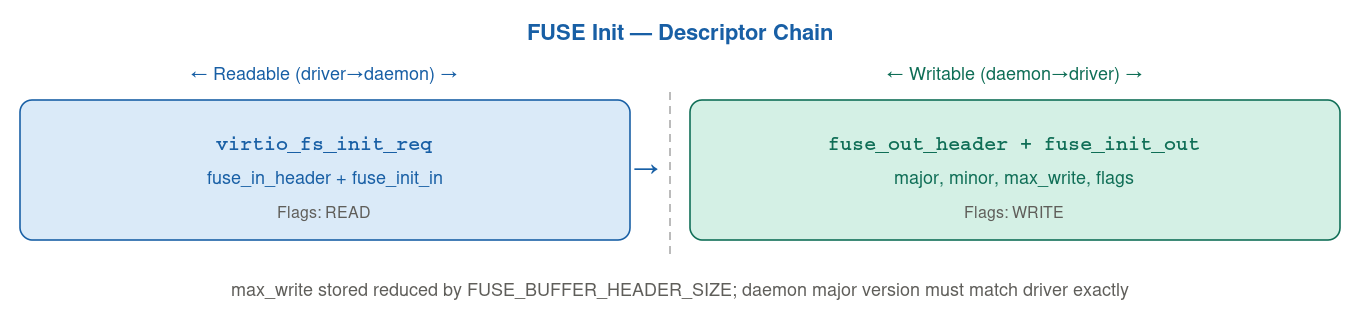
\includegraphics[width=0.90\linewidth]{init_chain.png}
  \caption{FUSE init chain: \texttt{virtio\_fs\_init\_req} carrying
    \texttt{fuse\_in\_header} and \texttt{fuse\_init\_in} (readable) |
    \texttt{fuse\_out\_header} and \texttt{fuse\_init\_out} with negotiated
    version and \texttt{max\_write} (writable).}
  \label{fig:init_chain}
\end{figure}

\subsection{Inode Resolution}

\texttt{\_lookup\_inode} sends a three-token \texttt{FUSE\_LOOKUP} chain:
request header (readable) | null-terminated path (readable) | response buffer
(writable).  The returned inode number, file handle, and seek offset are stored
in \texttt{\_fd\_info\_map} keyed by the POSIX descriptor integer, eliminating
repeated lookups for an open file.

\begin{figure}[htbp]
  \centering
  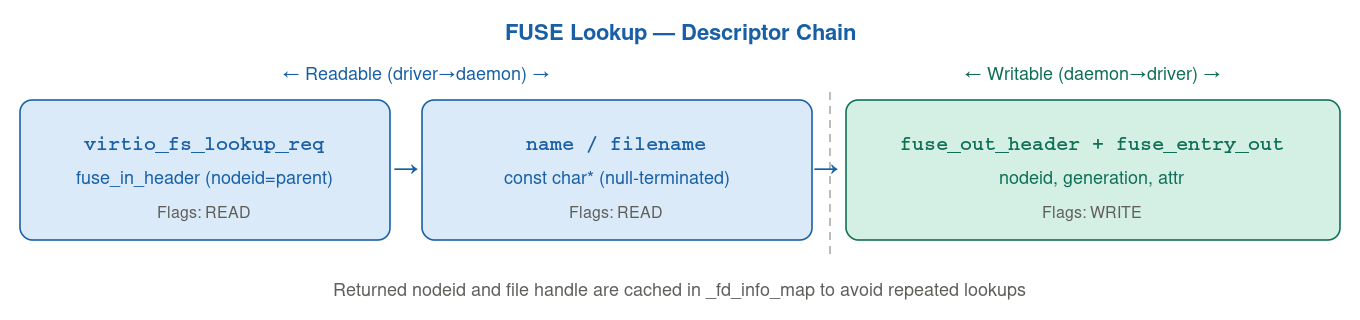
\includegraphics[width=0.90\linewidth]{lookup_chain.png}
  \caption{FUSE lookup chain: \texttt{virtio\_fs\_lookup\_req} with parent
    \texttt{nodeid} (readable) | null-terminated filename (readable) |
    \texttt{fuse\_out\_header} and \texttt{fuse\_entry\_out} with child inode
    attributes (writable).}
  \label{fig:lookup_chain}
\end{figure}

\subsection{Open, Create, and Close}

\texttt{\_open\_exist} calls \texttt{\_lookup\_inode} then issues
\texttt{FUSE\_OPEN}, storing the file handle with initial seek offset zero.
\texttt{\_open\_creat} issues \texttt{FUSE\_CREATE} against the root inode,
combining lookup and open in one round-trip.  \texttt{close} sends
\texttt{FUSE\_RELEASE} on the request queue, removes the descriptor from
\texttt{\_fd\_info\_map}, then sends \texttt{FUSE\_FORGET} on the high-priority
queue to promptly decrement the daemon's inode reference count.

\begin{figure}[htbp]
  \centering
  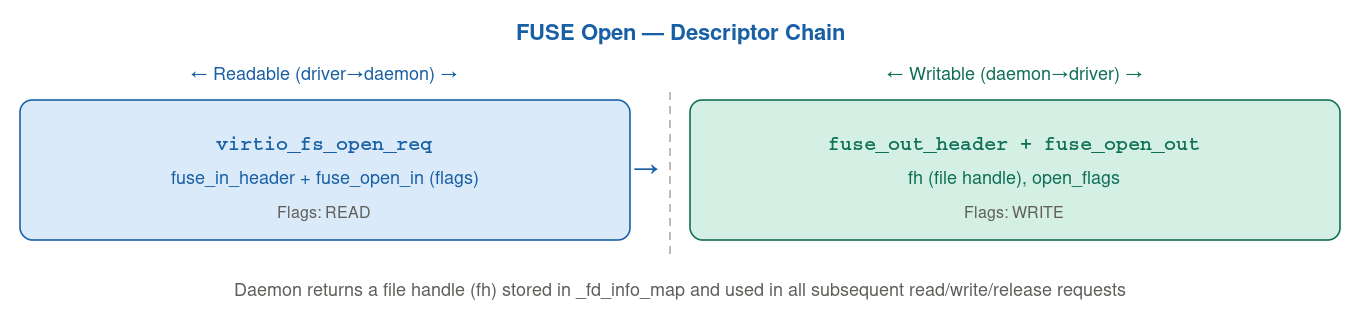
\includegraphics[width=0.90\linewidth]{open_chain.png}
  \caption{FUSE open chain: \texttt{virtio\_fs\_open\_req} carrying
    \texttt{fuse\_in\_header} and \texttt{fuse\_open\_in} (readable) |
    \texttt{fuse\_out\_header} and \texttt{fuse\_open\_out} with file handle
    and open flags (writable).}
  \label{fig:open_chain}
\end{figure}

\begin{figure}[htbp]
  \centering
  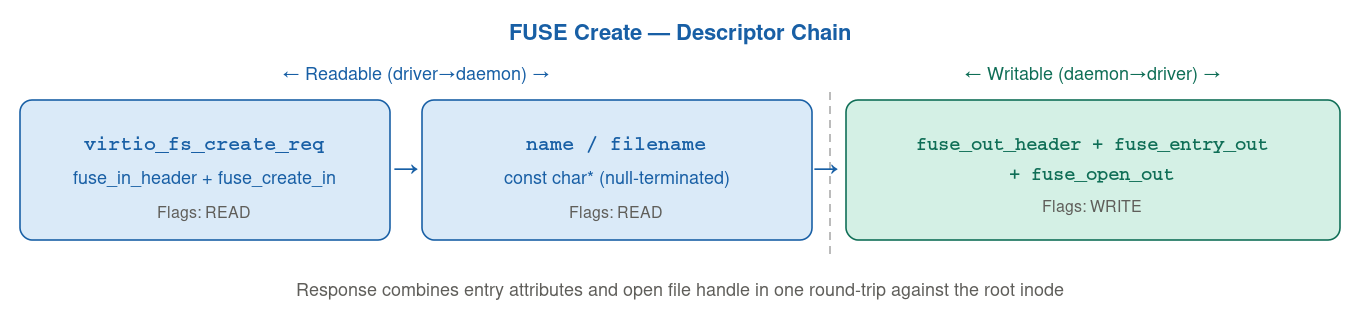
\includegraphics[width=0.90\linewidth]{create_chain.png}
  \caption{FUSE create chain: \texttt{virtio\_fs\_create\_req} with
    \texttt{fuse\_create\_in} (readable) | null-terminated filename (readable)
    | \texttt{fuse\_out\_header}, \texttt{fuse\_entry\_out}, and
    \texttt{fuse\_open\_out} combined in one writable descriptor, delivering
    both inode attributes and a file handle in a single round-trip.}
  \label{fig:create_chain}
\end{figure}

\begin{figure}[htbp]
  \centering
  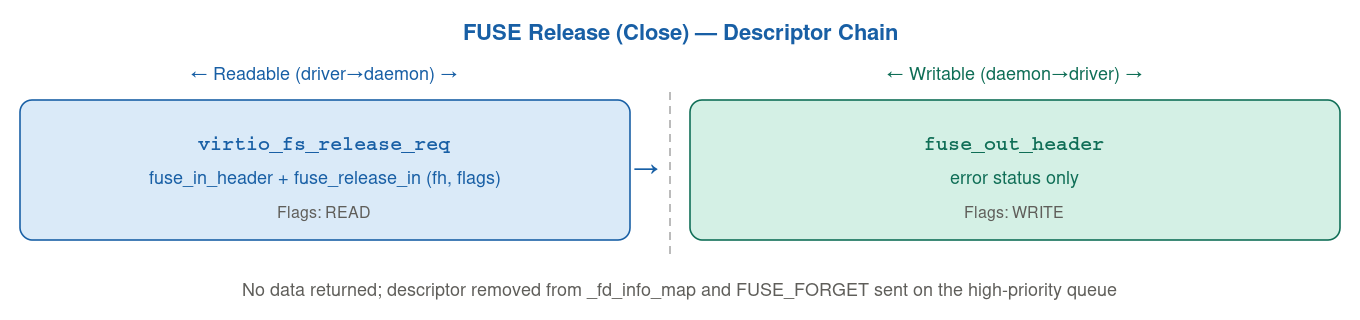
\includegraphics[width=0.90\linewidth]{release_chain.png}
  \caption{FUSE release (close) chain: \texttt{virtio\_fs\_release\_req}
    carrying \texttt{fuse\_release\_in} with the file handle and flags
    (readable) | \texttt{fuse\_out\_header} with error status only (writable).
    After the response the descriptor is removed from \texttt{\_fd\_info\_map}
    and \texttt{FUSE\_FORGET} is sent on the high-priority queue.}
  \label{fig:release_chain}
\end{figure}

\subsection{Read and Write}

All read and write operations deliver caller buffers directly to VirtioFSD via
Virtio descriptor chains with no intermediate copy.

\begin{figure}[htbp]
  \centering
  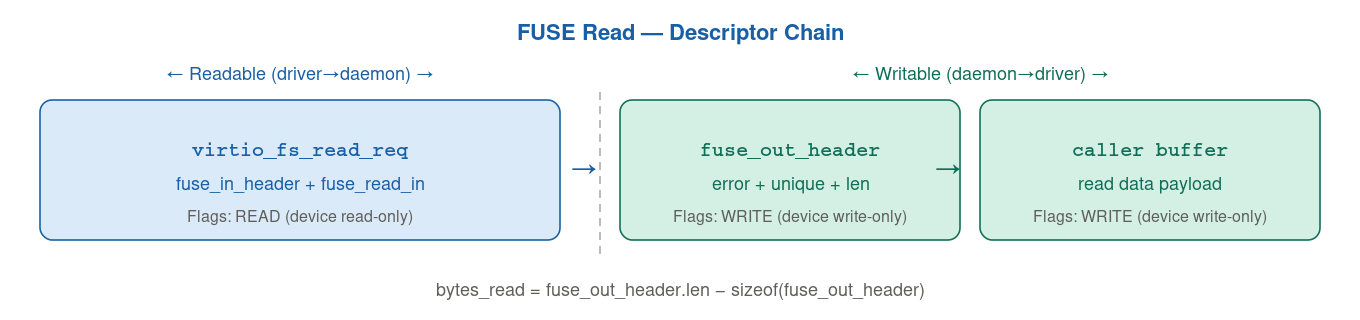
\includegraphics[width=0.90\linewidth]{read_chain.png}
  \caption{FUSE read chain: request header (readable) | response header
    (writable) | caller buffer (writable).  Bytes read =
    \texttt{fuse\_out\_header.len} $-$ \texttt{sizeof(fuse\_out\_header)}.}
  \label{fig:read_chain}
\end{figure}

\begin{figure}[htbp]
  \centering
  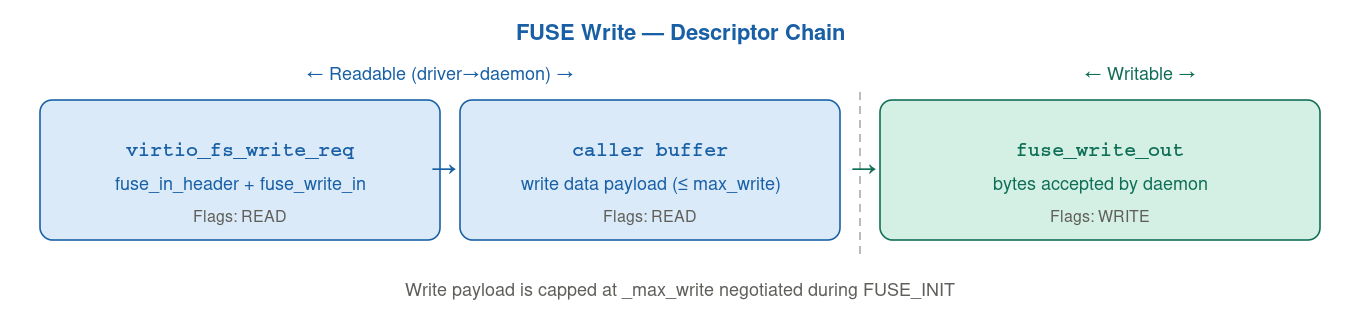
\includegraphics[width=0.90\linewidth]{write_chain.png}
  \caption{FUSE write chain: request header (readable) | caller buffer
    (readable, capped at \texttt{\_max\_write}) | \texttt{fuse\_write\_out}
    (writable).}
  \label{fig:write_chain}
\end{figure}

\begin{figure}[htbp]
  \centering
  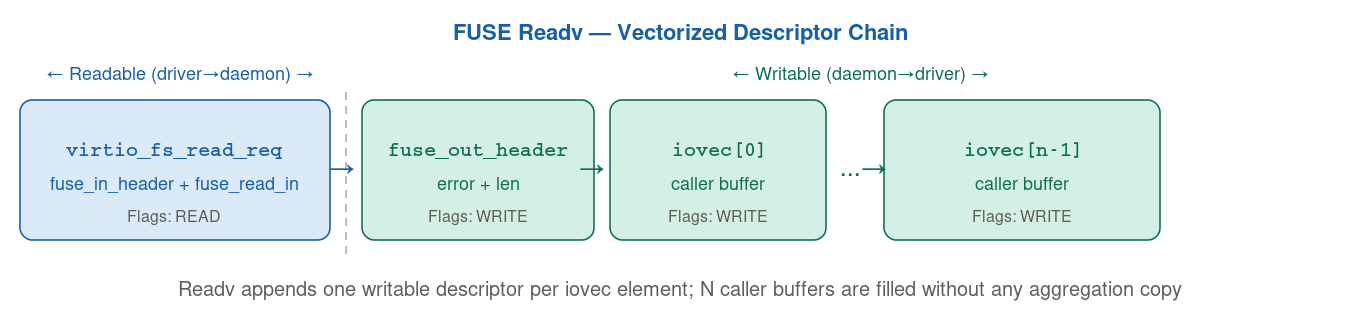
\includegraphics[width=0.90\linewidth]{readv_chain.png}
  \caption{FUSE vectorised read chain: request header (readable) |
    \texttt{fuse\_out\_header} (writable) | \texttt{iovec[0]} \ldots
    \texttt{iovec[n-1]} (writable) --- one descriptor per \texttt{iovec}
    element, allowing the device to scatter output directly into
    discontiguous caller buffers.}
  \label{fig:readv_chain}
\end{figure}

\begin{figure}[htbp]
  \centering
  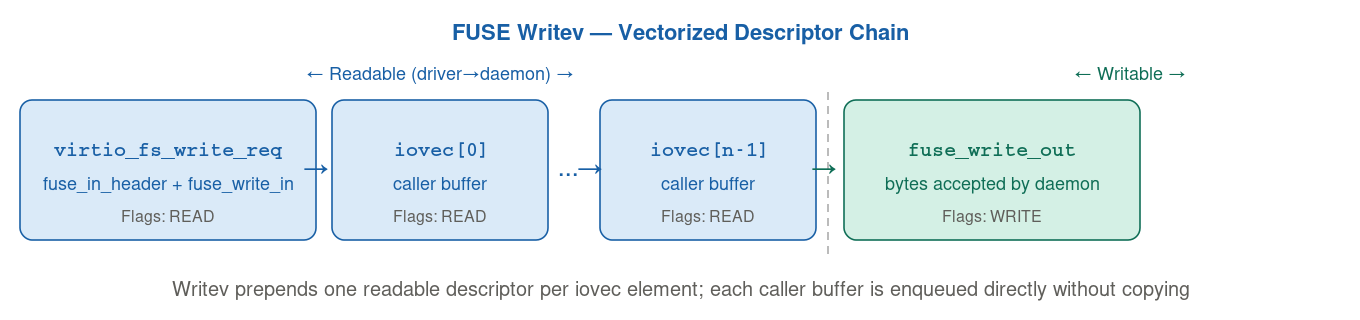
\includegraphics[width=0.90\linewidth]{writev_chain.png}
  \caption{FUSE vectorised write chain: request header (readable) |
    \texttt{iovec[0]} \ldots \texttt{iovec[n-1]} (readable) |
    \texttt{fuse\_write\_out} (writable) --- one descriptor per
    \texttt{iovec} element, gathering data from discontiguous caller
    buffers without an aggregation copy.  The combined byte size of all
    \texttt{iovec} elements must not exceed \texttt{\_max\_write}.}
  \label{fig:writev_chain}
\end{figure}

% I hate the colors
% Also, maybe structs

% Things are sort of hacked several places hmm. Should I really clean up and the repos?

The scatter-gather variants \texttt{readv} and \texttt{writev} append one
\texttt{VirtToken} per \texttt{iovec} element, exploiting descriptor chaining to
fill or drain discontiguous caller buffers with no aggregation buffer.
The combined byte size of all \texttt{iovec} elements must not exceed
\texttt{\_max\_write}, the negotiated per-request write limit exposed by the
device; the driver enforces this constraint before constructing the chain so
that the host never receives a request larger than it has agreed to handle.

\subsection{Seek}

\texttt{lseek} updates \texttt{\_fd\_info\_map}'s offset for
\texttt{SEEK\_SET} and \texttt{SEEK\_CUR} without issuing any Virtio operations
--- all offset state is authoritative in the driver.

\subsection{Unlink}

\texttt{unlink} issues \texttt{FUSE\_UNLINK} with the path pointer offset by
one byte to strip the leading path separator added by the VFS layer.  The
descriptor chain uses three entries: the first readable descriptor carries the
fixed \texttt{fuse\_in\_header} inside \texttt{virtio\_fs\_unlink\_req}; the
second readable descriptor points to the null-terminated name string (with
the $+1$ offset applied); the daemon writes back only a
\texttt{fuse\_out\_header} containing the error code in the single writable
descriptor.

\begin{figure}[htbp]
  \centering
  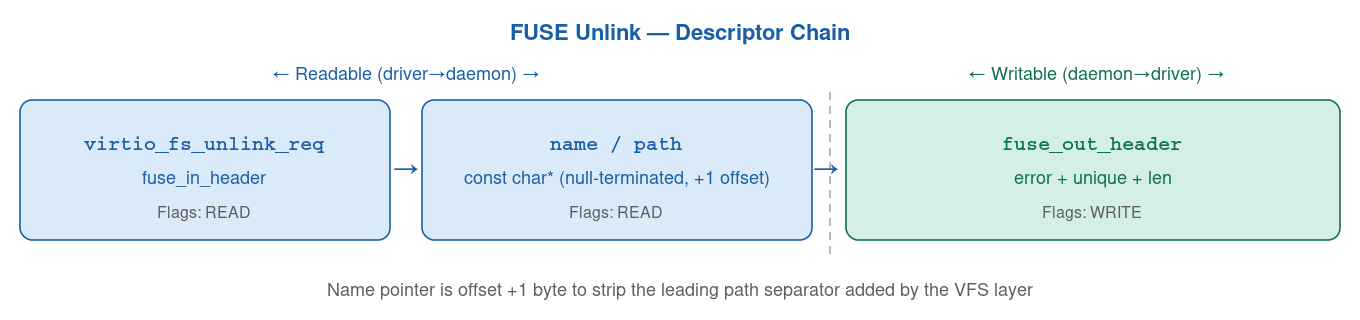
\includegraphics[width=0.90\linewidth]{unlink_chain.png}
  \caption{FUSE unlink chain: \texttt{virtio\_fs\_unlink\_req} carrying the
    fixed \texttt{fuse\_in\_header} (readable) | \texttt{name/path} string as a
    separate readable descriptor (pointer offset $+1$ to strip the leading
    separator added by the VFS layer) | \texttt{fuse\_out\_header} (writable).}
  \label{fig:unlink_chain}
\end{figure}

% ════════════════════════════════════════════════════════════════════════════
%  CHAPTER 5 — EVALUATION
% ════════════════════════════════════════════════════════════════════════════
\chapter{Evaluation}
\label{chap:evaluation}

This chapter presents the experimental evaluation of the VirtioFS implementation
for IncludeOS.  Three research questions are investigated through a set of
controlled microbenchmarks and an end-to-end application workload.
Section~\ref{sec:setup} describes the common infrastructure shared by all
experiments.  Sections~\ref{sec:rq1}--\ref{sec:rq3} then present the setup,
results, and analysis for each research question in turn.

\section{Experimental Setup}
\label{sec:setup}

\subsection{Virtual-Machine Infrastructure}

All experiments are executed inside virtual machines managed by QEMU/KVM on the
same host workstation, ensuring that CPU microarchitecture and memory topology
are constant across every run.  A shared host directory is exposed to the guest
through VirtioFS, the primary transport under evaluation. The host directory itself is mounted on a \textbf{tmpfs} ramdisk so that host-side storage latency and caching effects are eliminated from the measurements. The VirtioFS daemon is launched with direct I/O passthrough (\textbf{---allow-direct-io}) for guest and daemon caching disabled (\textbf{---cache never}).

\textbf{IncludeOS} machines run with a single virtual processor and 3 gibibytes of ram. Benchmark code and IncludeOS are linked and bundled into a bootable image. The experiments are executed with two VirtioFS driver configurations:

\paragraph{Polling.} After submitting a request to the VirtioFS virtqueue, the
IncludeOS driver busy-polls the used-ring until the host returns
a completion.  No interrupt is taken and the vCPU never halts.

\begin{lstlisting}[caption=Busy-polling,style=chstyle,language=C]
_req.enqueue(tokens);
while(_req.has_processed_used()); // Busy-polling
_req.dequeue();
\end{lstlisting}

\paragraph{IRQ (MSI-X).} After submission, the vCPU executes a \texttt{HLT}
instruction and sleeps until a MSI-X interrupt from the VirtioFS device
signals completion. We register a dummy function as the deferred callback routine for the request virtqueue. Using interrupts frees the virtual processor for other work, reduces energy and CPU utilization, but introduces extra latency compared to busy-polling.

\begin{lstlisting}[caption=VirtioFS deferred interrupt setup,style=chstyle,language=C]
// VirtioFS init function
_control.enable_msix(1);
auto event_num = Events::get().subscribe(
  {this, &VirtioFS_device::_fuse_log_reply}
);
d.setup_msix_vector(0, IRQ_BASE + event_num);
_control.set_driver_ok_bit();

// Enable_msix function
uint8_t Virtio_control::enable_msix(uint8_t required_msix_count) {
  if (required_msix_count > 0) {
    _msix_enabled = true;

    /* Grabbing PCI resources. Dependency for MSIX code */
    _pcidev.probe_resources();
    _pcidev.parse_capabilities();

    /* Checking for the availablity of MSIX capability */
    bool supports_msix = _pcidev.msix_cap() > 0;
    CHECK(supports_msix, "Device supports MSIX!");
    _virtio_panic(supports_msix);

    /* Driver requires required_msix_count # of vectors */
    _pcidev.init_msix();
    uint8_t msix_vector_count = _pcidev.get_msix_vectors();
    bool sufficient_msix_count = msix_vector_count >= required_msix_count;
    CHECK(sufficient_msix_count, "Sufficient msix vector count (%d)", msix_vector_count);
    _virtio_panic(sufficient_msix_count);

    return msix_vector_count;
  }

// Split queue setting the MSI-X vector
cfg.queue_msix_vector = VIRTIO_MSI_NO_VECTOR;
\end{lstlisting}

% TODO: Add how this works with my Virtio stuff :) (code listing)

\textbf{Linux} machines execute with four virtual processors and 8 gibibytes of ram. The machines run with more resources to reduce the scheduling and memory pressure from other processes running on the system. The benchmark processes run with minimal interference.

\subsection{Timing}

All benchmarks use the same \textbf{chrono::high\_resolution\_clock} clock in C++ for timestamps. The benchmarks calculate the time delta before and after the function to be timed.

\subsection{Reproducible Builds}

All benchmark programs are compiled with the Nix package manager to guarantee
bit-for-bit reproducibility across machines.

IncludeOS unikernel binaries are built with
\texttt{includeos.stdenv.mkDerivation}; the resulting
\texttt{virtiofs\_bench.elf.bin} image is passed directly to the
\texttt{boot} launcher.  Linux binaries are compiled with the \texttt{pkgsMusl}
static C library toolchain to minimize runtime dependencies and prevent dynamic
linker behavior from confounding results.

\subsection{Host machine}

The machine is \texttt{Lenovo LOQ 15AHP10} laptop running a \texttt{AMD Ryzen 7 250 (8 cores and 16 threads)} with 32GiB of RAM. The host operating system is \textbf{Debian 13 (Trixie)} with the kernel version \textbf{6.12.63}.

\subsection{POSIX I/O Benchmark (Experiments 1 \& 2)}
\label{sec:posix_setup}

The synchronous-I/O benchmark exercises VirtioFS through the standard POSIX file
API (\texttt{open}/\texttt{read}/\texttt{write}/\texttt{lseek}/\texttt{close}).
In IncludeOS this translates directly into driver calls with no kernel syscall
boundary; in Linux the calls traverse the VFS and protections mechanims before reaching
the \texttt{virtiofsd}-backed driver.

A 200~MiB binary file (\texttt{syncio\_testing\_file.bin}) pre-placed on the shared \texttt{tmpfs}
serves as the read source. Write benchmarks create a fresh output file on each
run and remove it afterwards. Files are opened with \texttt{O\_DIRECT} to bypass the page cache.

The benchmark iterates over chunk sizes from 8~KiB to
248~KiB in steps of 8~KiB (31 sizes).  For each chunk size 30 independent runs
are executed.  Four access patterns are measured: \emph{sequential read},
\emph{sequential write}, \emph{random read}, and \emph{random write}.  The
random benchmarks permute chunk indices with a fixed seed (Mersenne Twister,
seed 42).

Each run calculates the time delta of the innermost processing
loop. The result is recorded as elapsed time in milliseconds and as throughput
in mebibytes per second (MiB/s), computed as $\text{filesize} / \text{elapsed}$.

\subsection{io\_uring Benchmark (Experiment 3)}
\label{sec:iouring_setup}

The io\_uring benchmark is equivalent to POSIX with applied io\_uring patches. The submission queue depth is set to 1; a single outstanding I/O is submitted and waited upon before the next is issued, matching the serialized access pattern of the POSIX benchmark. io\_uring is configured with a polling kernel thread using \texttt{IORING\_SETUP\_SQPOLL}. This spawns a kernel thread that polls the submission queue without requiring a \texttt{io\_uring\_enter} system call from the application. This benchmark runs only on Linux. 

\subsection{C63 Video Decoder Benchmark}
\label{sec:c63dec_setup}

The c63 codec is a simplified video codec developed for educational
purposes. C63 uses buffered file I/O that calls vectorized I/O.

The decoder \texttt{c63dec} reads a compressed \texttt{.c63} file
from the VirtioFS-mounted directory and writes the decoded raw YUV frames back
to the same directory, exercising both the read and write paths of the VirtioFS
driver under a realistic, compute-bound workload.

The input file is a 60-frame encoded of West Wind Easy (\texttt{wwe.c63}).
The entire decode-and-write sequence is timed with
\texttt{std::chrono::high\_resolution\_clock} and repeated 30 times per system
configuration.  Run~0 is treated as a cold-start observation and excluded from
statistical analysis; runs~1--29 are used to compute means and confidence
intervals.

% A custom stack allocator is used to 

Three system configurations are compared: Linux, IncludeOS Polling, and
IncludeOS IRQ.

\section{RQ1 -- VirtioFS Throughput: IncludeOS vs.\ Linux}
\label{sec:rq1}

\textbf{RQ1:} \emph{Can a VirtioFS implementation in IncludeOS have a higher I/O
throughput than Linux?}

\subsection{Results}

Figure~\ref{fig:rq1_combined} shows the mean throughput (with 95\% confidence
intervals as shaded bands) across all 31 chunk sizes for the four access
patterns, comparing Linux POSIX, IncludeOS Polling, and IncludeOS IRQ.
Figure~\ref{fig:rq1_peak} summarises peak throughput as a bar chart.

\begin{figure}[htbp]
  \centering
  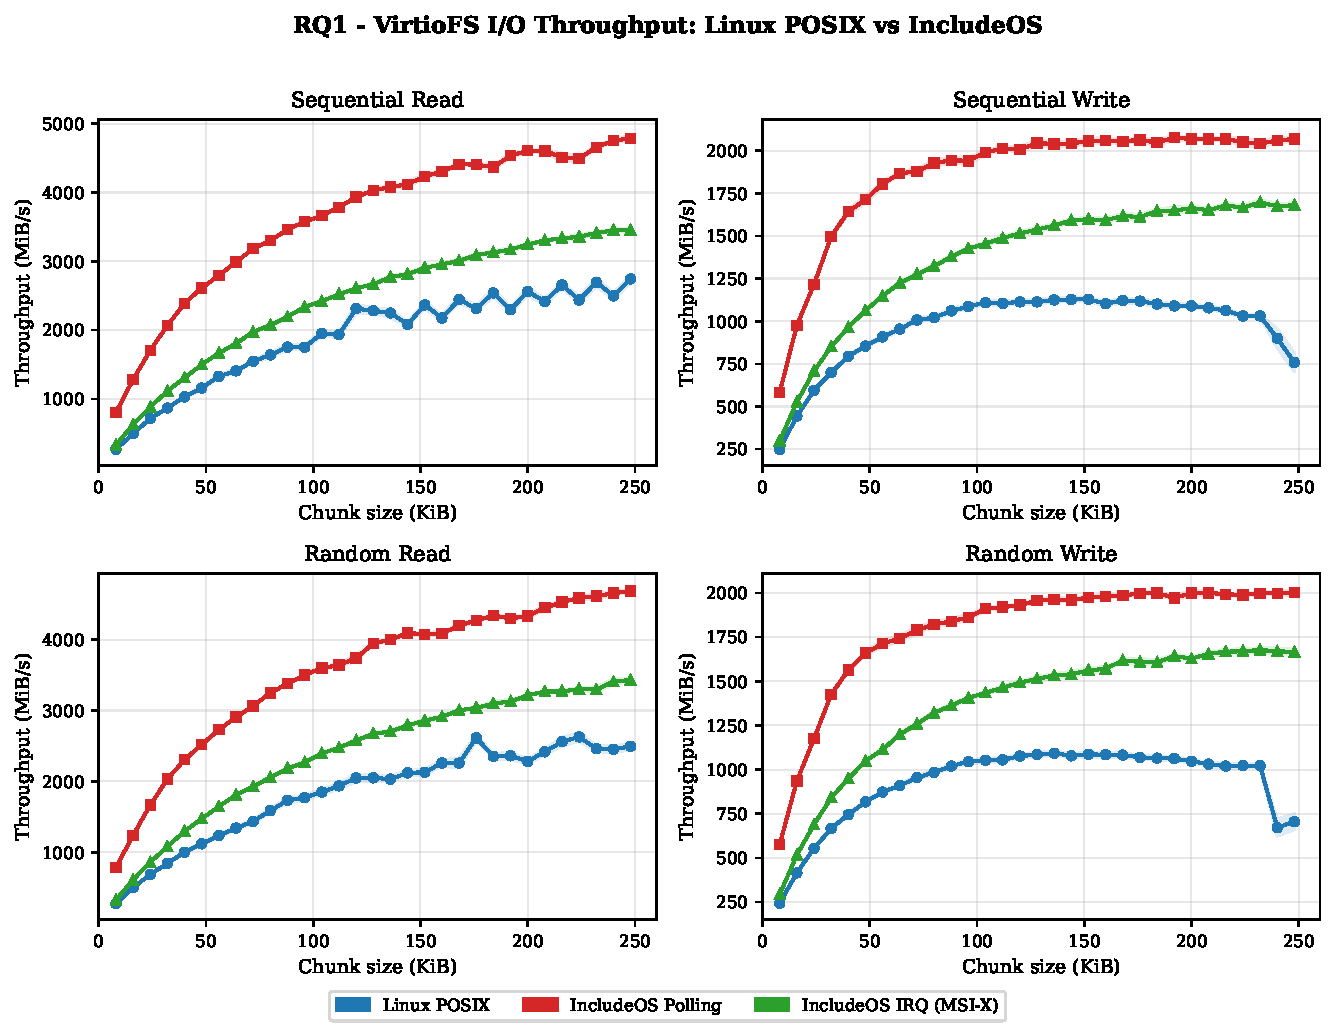
\includegraphics[width=\linewidth]{rq1_combined.pdf}
  \caption{RQ1 -- Mean VirtioFS throughput (MiB/s) vs.\ chunk size for all four
    access patterns.  Shaded bands represent 95\% confidence intervals over 30
    runs.}
  \label{fig:rq1_combined}
\end{figure}

% \begin{figure}[htbp]
%   \centering
%   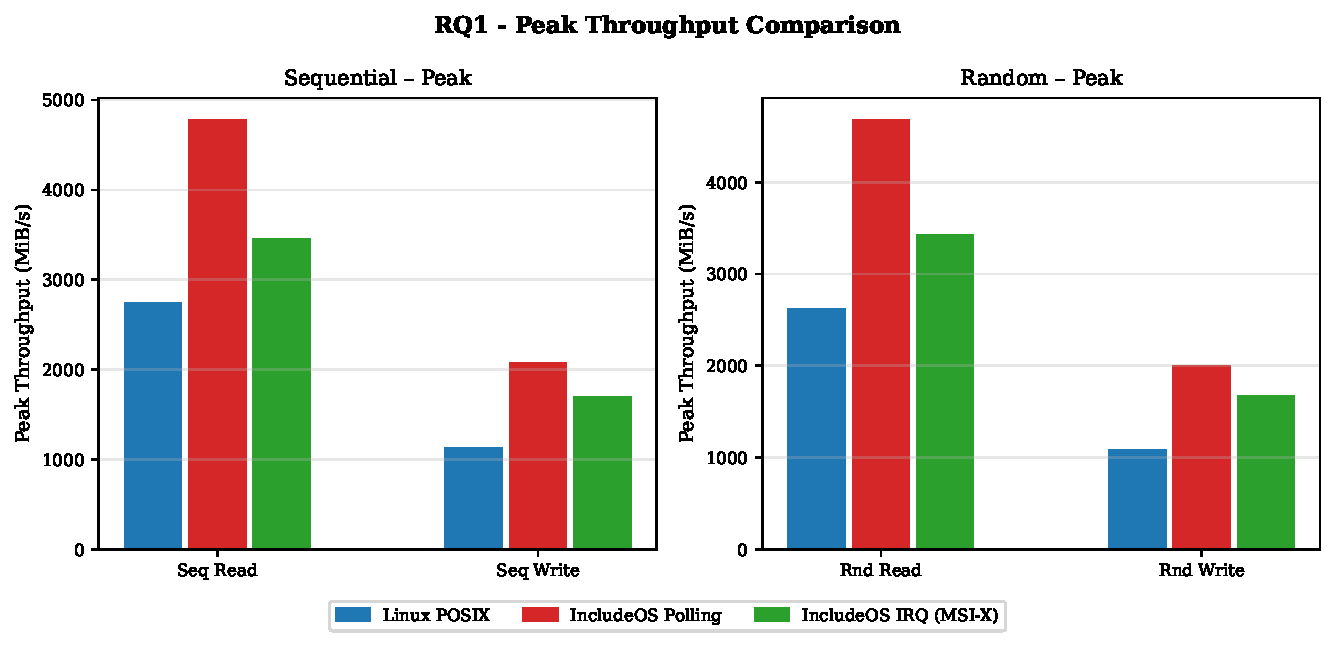
\includegraphics[width=\linewidth]{rq1_peak_bar.pdf}
%   \caption{RQ1 -- Peak throughput comparison for sequential (left) and random
%     (right) I/O across the three system configurations.}
%   \label{fig:rq1_peak}
% \end{figure}

\paragraph{IncludeOS Polling vs.\ Linux POSIX.}
IncludeOS Polling achieves the highest throughput across every access pattern and
chunk size.  At peak (248~KiB chunks for reads, around 192--248~KiB for writes),
it sustains \textbf{4,786~MiB/s} for sequential reads and \textbf{2,076~MiB/s}
for sequential writes --- representing speedups of $\times$\textbf{1.74} and
$\times$\textbf{1.84} over the Linux POSIX baseline respectively.  Random access
exhibits nearly identical relative gains: $\times$1.78 for random reads and
$\times$1.83 for random writes.

The advantage is even more pronounced at small chunk sizes, where system call and
interrupt overhead dominate.  At 8~KiB chunks, IncludeOS Polling delivers
\textbf{804~MiB/s} for sequential reads against only \textbf{266~MiB/s} for
Linux POSIX --- a $\times$\textbf{3.02} speedup.  This highlights how the
elimination of the kernel-mode/user-mode transition, the VFS dispatch, and the
FUSE/\texttt{virtiofsd} round-trip dramatically reduces per-request latency when
requests are frequent and small.

\paragraph{IncludeOS IRQ vs.\ Linux POSIX.}
IncludeOS IRQ outperforms Linux POSIX across the entire chunk range, but by a
narrower margin than polling.  Peak sequential read throughput reaches
\textbf{3,454~MiB/s} ($\times$1.26 over Linux POSIX), and peak sequential write
reaches \textbf{1,696~MiB/s} ($\times$1.50).  At 8~KiB chunks the IRQ mode
achieves $\times$1.24 over Linux for sequential reads.

The performance gap between IRQ and Polling within IncludeOS is itself
instructive.  Polling outperforms IRQ by $\times$1.39 at peak sequential read
and $\times$1.22 at peak sequential write.  This gap is attributable to the
round-trip cost of MSI-X delivery: after every \texttt{HLT}, the vCPU must be
woken from its halted state by the hypervisor before execution can resume, a path
that involves an exit from the guest, interrupt injection, and a re-entry.

\paragraph{Throughput scaling with chunk size.}
All three systems exhibit a consistent pattern: throughput rises steeply from
8~KiB and plateaus beyond approximately 128--192~KiB, after which there is
little additional gain from larger transfers.  This plateau reflects the
saturation of the underlying \texttt{tmpfs} memory bandwidth.  The plateau for
IncludeOS Polling, however, sits roughly twice as high as that for Linux POSIX.

\subsection{Analysis}

The throughput advantage of IncludeOS over Linux can be attributed to three
structural differences:

\begin{enumerate}
  \item \textbf{No syscall overhead.}  In IncludeOS, a call to \texttt{read()}
    or \texttt{write()} dispatches directly to the VirtioFS driver without a
    privilege-level switch and additional layers.

  \item \textbf{Absence of OS interference.}  As a unikernel, IncludeOS runs a
    single cooperative task. There is no scheduler preemption overhead during the benchmark.
\end{enumerate}

\textbf{Answer to RQ1:} Yes.  The IncludeOS VirtioFS implementation achieves
substantially higher I/O throughput than Linux across all measured access
patterns, chunk sizes, and notification modes.  In polling mode the peak speedup
reaches $\times$1.74--1.84 at large chunk sizes and $\times$2.34--3.02 at
8~KiB.

\section{RQ2 -- Tweaking Linux: io\_uring SQPOLL}
\label{sec:rq2}

\textbf{RQ2:} \emph{Why is the I/O throughput in VirtioFS Linux slower than
IncludeOS?  Can we tweak Linux to achieve equivalent performance?}

\subsection{Results}

Figure~\ref{fig:rq2_combined} compares Linux POSIX and Linux io\_uring SQPOLL
across the four access patterns.  Figure~\ref{fig:rq2_speedup} shows the
per-chunk-size speedup ratio of io\_uring relative to POSIX.

\begin{figure}[htbp]
  \centering
  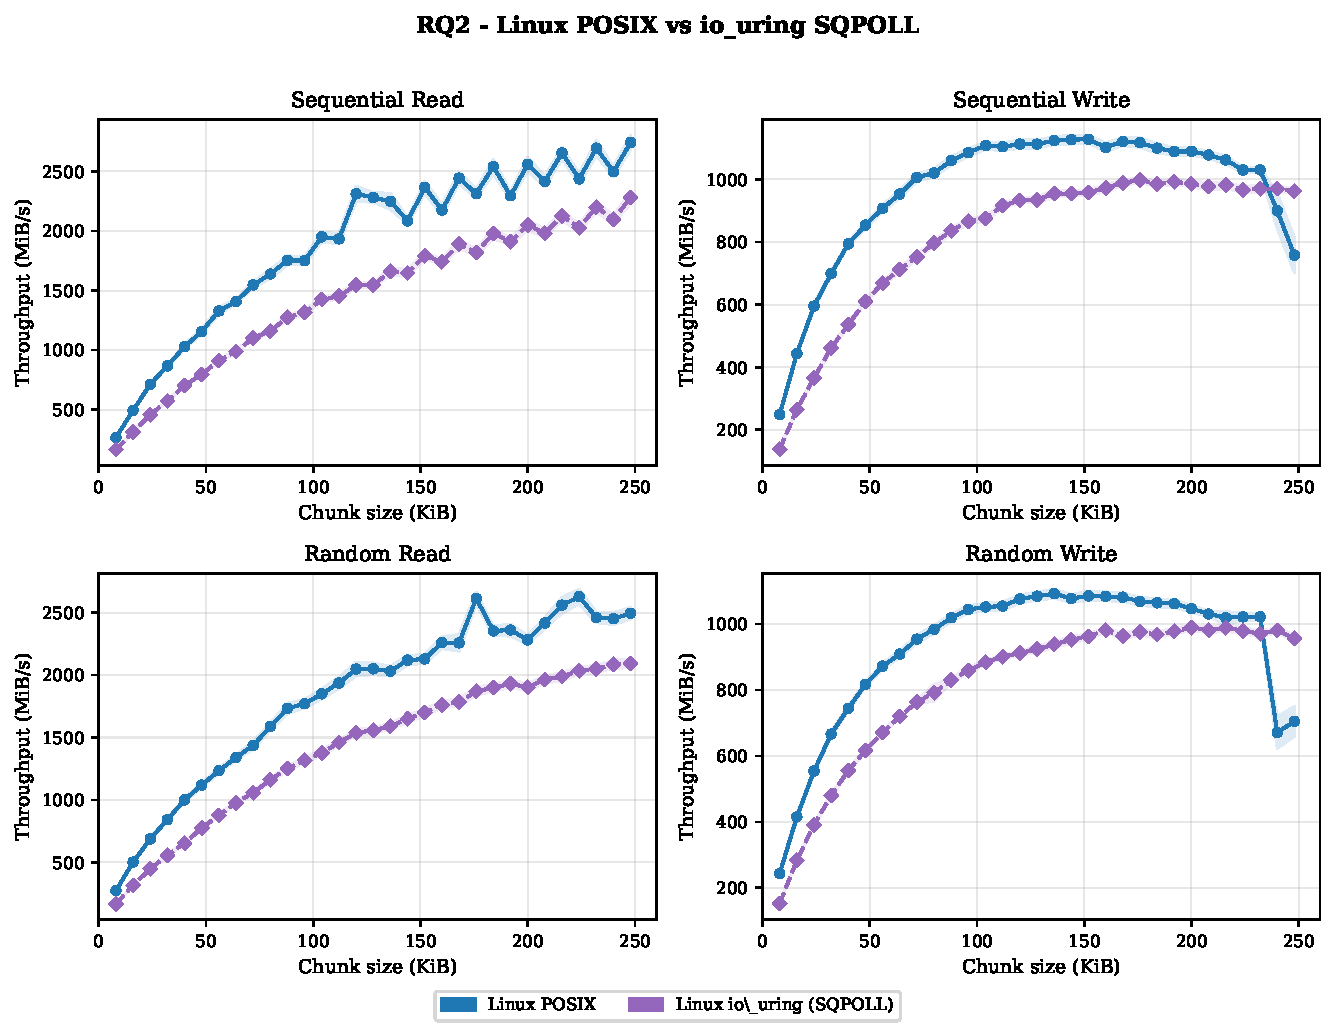
\includegraphics[width=\linewidth]{rq2_combined.pdf}
  \caption{RQ2 -- Mean VirtioFS throughput: Linux POSIX vs.\ Linux io\_uring
    SQPOLL.  Shaded bands are 95\% confidence intervals.}
  \label{fig:rq2_combined}
\end{figure}

\begin{figure}[htbp]
  \centering
  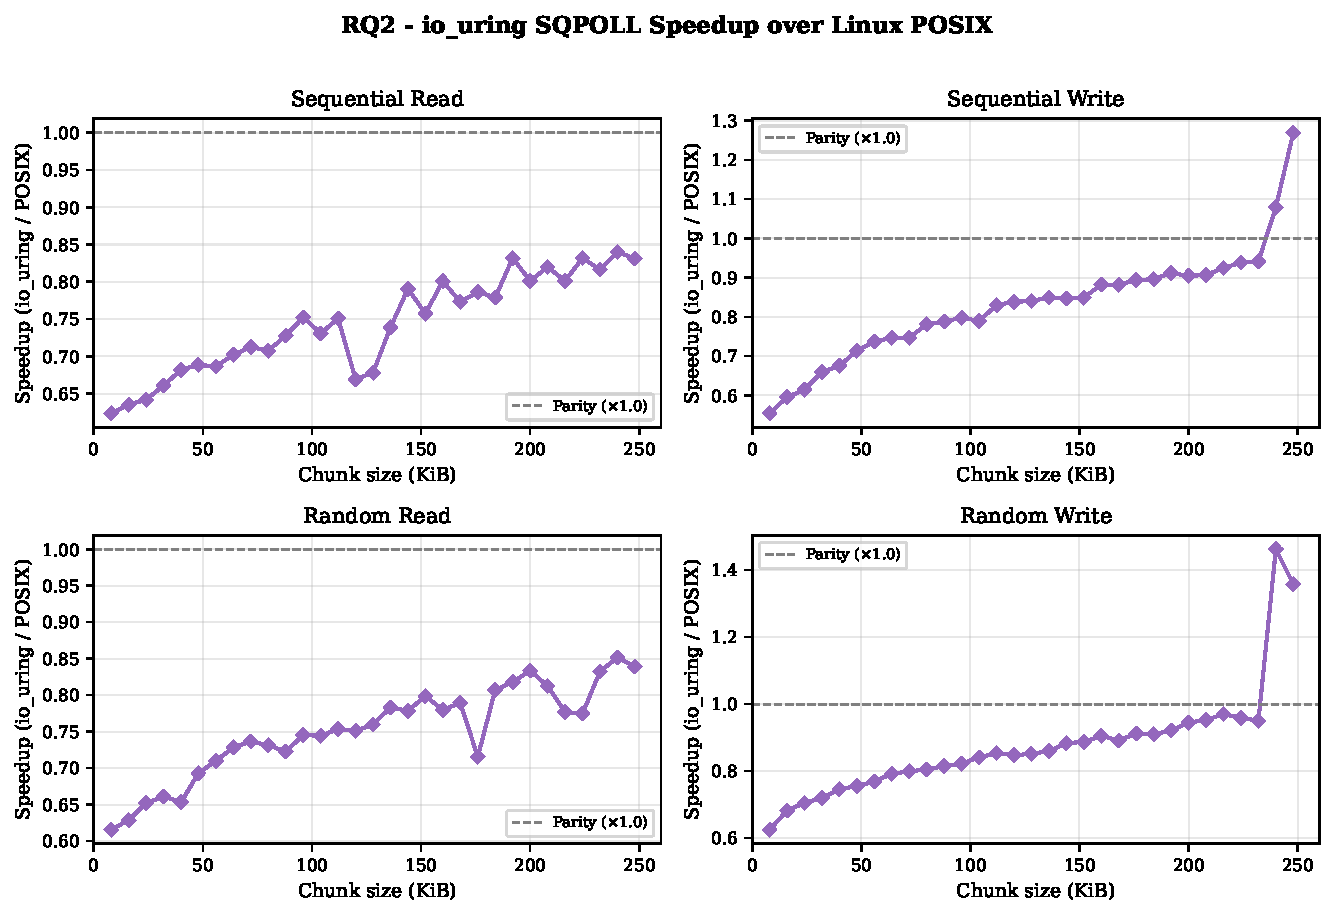
\includegraphics[width=\linewidth]{rq2_speedup.pdf}
  \caption{RQ2 -- io\_uring SQPOLL throughput as a ratio of Linux POSIX
    throughput (values above 1.0 indicate an improvement, below 1.0 a
    regression).  The dashed grey line marks parity.}
  \label{fig:rq2_speedup}
\end{figure}

Contrary to expectations, io\_uring SQPOLL is \emph{slower} than Linux POSIX
across the entire chunk-size range and all four access patterns.  Peak sequential
read throughput with io\_uring reaches only \textbf{2,280~MiB/s} versus
\textbf{2,743~MiB/s} for POSIX (a regression of $\times$0.83).  For sequential
writes the regression is $\times$0.88.  At the smallest chunk size of 8~KiB, the
penalty is even larger: io\_uring achieves only \textbf{166~MiB/s} for
sequential reads, against \textbf{266~MiB/s} for POSIX ($\times$0.62).

Figure~\ref{fig:all_systems} places all four configurations side by side to
contextualise these findings relative to the IncludeOS baselines.

\begin{figure}[htbp]
  \centering
  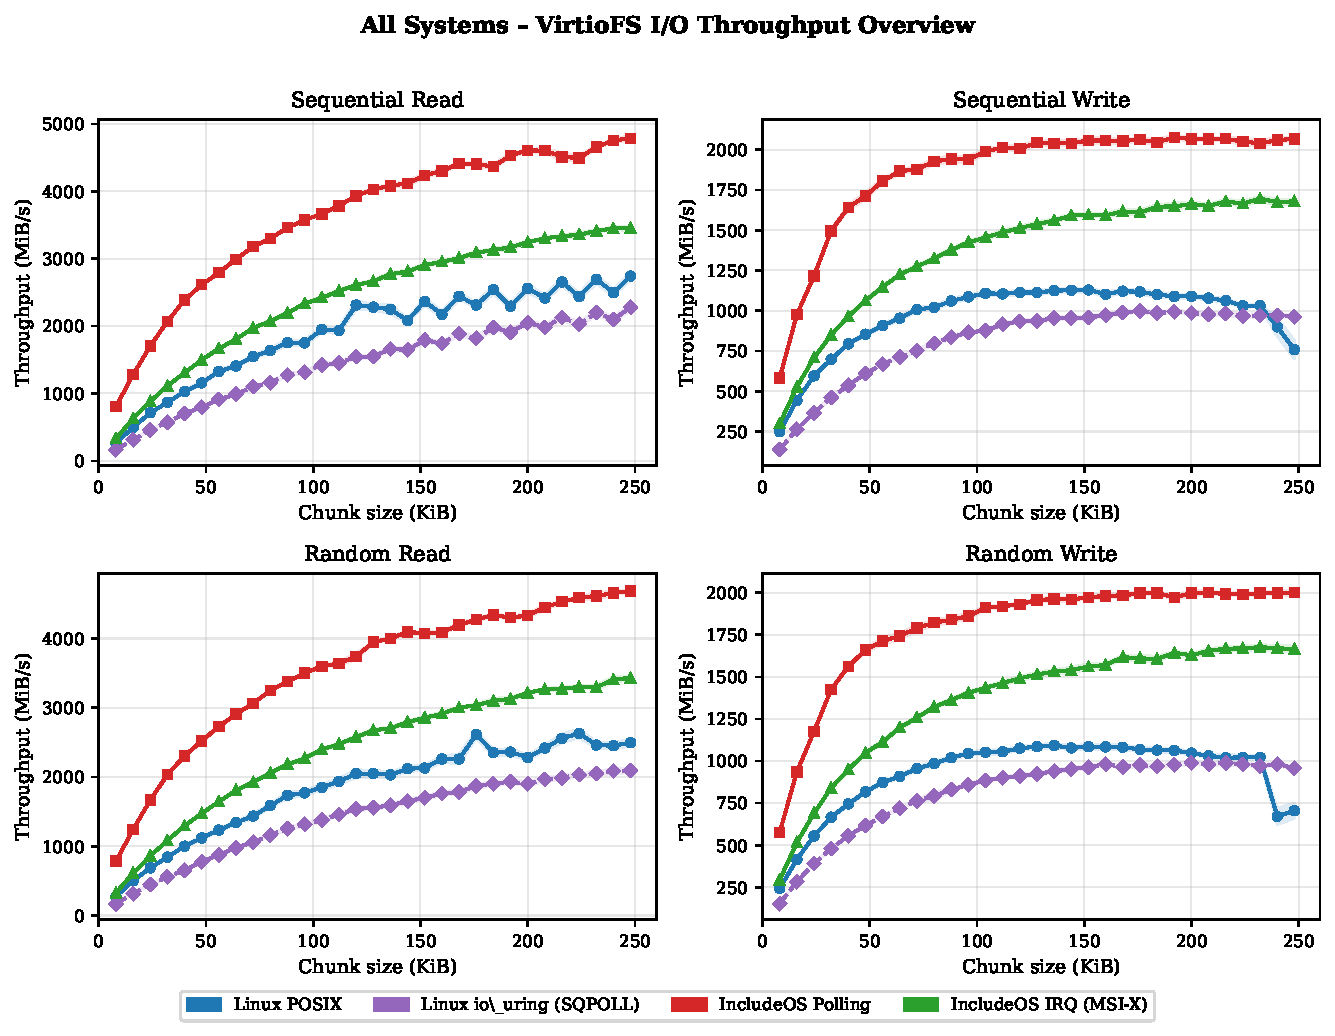
\includegraphics[width=\linewidth]{all_systems_combined.pdf}
  \caption{All system configurations -- VirtioFS throughput overview for all
    four access patterns.  io\_uring falls below even the Linux POSIX baseline.}
  \label{fig:all_systems}
\end{figure}

\subsection{Analysis}

\paragraph{Queue depth of 1.}  The benchmark deliberately maintains a single
outstanding I/O at a time. SQPOLL provides its greatest benefit at high queue
depths where many I/O operations can be batched into the submission ring with a
single kernel notification. At depth 1 the overhead of ring management is
incurred for every single operation without amortization.

\textbf{Answer to RQ2:}  The throughput gap between Linux and IncludeOS is
caused by the multiple software layers interposed between the application and the
VirtioFS virtqueue: system calls, the VFS, FUSE framing, and the
\texttt{virtiofsd} user-space daemon.  Replacing synchronous POSIX calls with
io\_uring SQPOLL does not close this gap; on the contrary, at queue depth~1 with VirtioFS, SQPOLL introduces a throughput regression of 9--38\%
compared with ordinary POSIX I/O.

\section{RQ3 -- Impact on Video Decoding}
\label{sec:rq3}

\textbf{RQ3:} \emph{What impact will enhanced I/O throughput have on common
tasks such as video decoding?}

\subsection{Results}

Figure~\ref{fig:rq3_box} shows a box plot of decode times (runs 1--29) for the
three system configurations.

% Figure~\ref{fig:rq3_bar} presents means with 95\% confidence intervals and speedup annotations relative to Linux.

\begin{figure}[htbp]
  \centering
  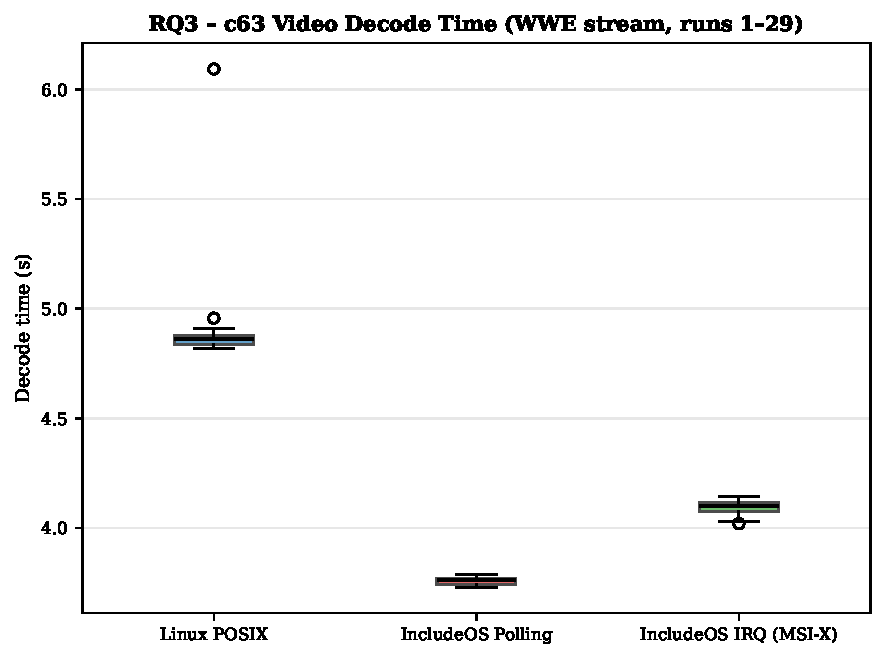
\includegraphics[width=0.8\linewidth]{rq3_c63dec_boxplot.pdf}
  \caption{RQ3 -- Distribution of c63 decode times over 29 warm runs.  Boxes
    span the interquartile range; whiskers extend to the most extreme
    non-outlier observation.}
  \label{fig:rq3_box}
\end{figure}

% I will also make a benchmark where I will interleave

% Reference the part of IRQ to 

% Mention that vectorized I/O is used here.
% Calculate how much of the time is actually decoding versus I/O
% This can be done by
% Throughput out

% \begin{figure}[htbp]
%   \centering
%   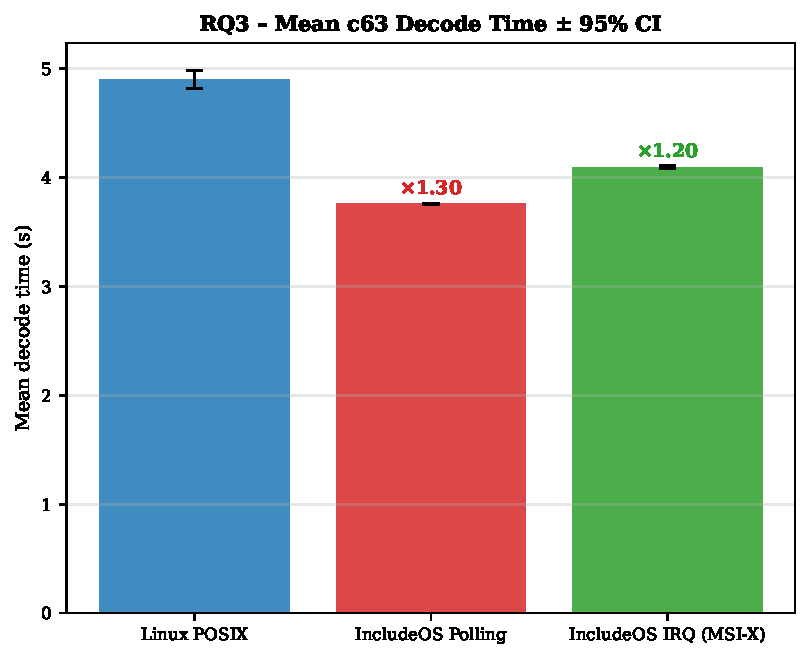
\includegraphics[width=0.7\linewidth]{rq3_c63dec_bar.pdf}
%   \caption{RQ3 -- Mean c63 decode time $\pm$ 95\% CI\@.  Speedup labels above
%     the IncludeOS bars are relative to the Linux mean.}
%   \label{fig:rq3_bar}
% \end{figure}

\begin{table}[htbp]
  \centering
  \caption{c63dec benchmark statistics (runs 1--29; run 0 excluded as cold
    start).  Speedup is relative to Linux POSIX.}
  \label{tab:c63dec_stats}
  \begin{tabular}{lrrrrc}
    \toprule
    \textbf{Configuration} & \textbf{Mean (s)} & \textbf{Std (s)} &
      \textbf{Min (s)} & \textbf{Max (s)} & \textbf{Speedup} \\
    \midrule
    Linux POSIX             & 4.861 & 0.032 & 4.820 & 4.957 & $\times$1.00 \\
    IncludeOS Polling       & 3.759 & 0.015 & 3.731 & 3.790 & $\times$\textbf{1.29} \\
    IncludeOS IRQ (MSI-X)   & 4.096 & 0.030 & 4.020 & 4.144 & $\times$1.19 \\
    \bottomrule
  \end{tabular}
\end{table}

\paragraph{IncludeOS Polling.}
IncludeOS Polling achieves a mean decode time of \textbf{3.759~s}, compared with
\textbf{4.861~s} for Linux POSIX --- a speedup of $\times$\textbf{1.29}, or a
\textbf{22.7\% reduction} in wall-clock decode time.

\paragraph{IncludeOS IRQ.}
IncludeOS IRQ reduces decode time to \textbf{4.096~s}, a $\times$\textbf{1.19}
speedup (18.6\% reduction) over Linux.  The 8.5\% gap between IRQ and Polling
within IncludeOS reflects the interrupt-delivery overhead noted in
Section~\ref{sec:rq1}: for a codec that issues many small I/O requests per
decoded frame, the accumulated cost of MSI-X wakeup cycles is significant.

\paragraph{Cold-start behaviour.}
Run~0 reveals a striking asymmetry between Linux and IncludeOS.  Linux requires
\textbf{6.092~s} on the cold run --- a \textbf{25.3\%} penalty over its warm
mean --- caused by page-fault handling, dynamic loader initialisation, and I/O
scheduling setup.  IncludeOS Polling's cold run takes \textbf{3.772~s}, only
\textbf{0.4\%} above its warm mean; IncludeOS IRQ shows a similarly negligible
\textbf{0.2\%} cold overhead.  This behaviour reflects the unikernel's
single-process, pre-linked execution model: there is no dynamic linker, no kernel
process initialisation, and no page-table population at startup.

\subsection{Analysis}

The magnitude of the end-to-end speedup (22.7\%) is smaller than the raw
peak-throughput speedup seen in the microbenchmarks ($\times$1.74 for sequential
reads).  This is expected: the c63dec workload is not I/O-bound.  A substantial
fraction of execution time is spent in the CPU decode pipeline (VLC decoding,
IDCT, motion compensation), which is identical across all configurations.  The
measured speedup therefore represents the I/O contribution to the total workload,
scaled by the Amdahl factor of the non-I/O fraction.

\textbf{Answer to RQ3:}  The higher I/O throughput of the IncludeOS VirtioFS
implementation translates directly into faster end-to-end execution of a
realistic video decoding task.  IncludeOS Polling completes decoding
\textbf{22.7\% faster} than Linux POSIX. The unikernel also eliminates the significant cold-start
penalty observed on Linux, making every execution faster and more predictable.

\section{Threats to Validity}
\label{sec:threats}

\paragraph{Internal validity.}
The \texttt{tmpfs} shared directory eliminates disk I/O from the measurements but
also places an upper bound on achievable throughput set by the host's DRAM
bandwidth.  Both Linux and IncludeOS are subject to the same bound; the relative
comparison remains valid, but absolute numbers cannot be directly extrapolated to
persistent storage scenarios.

\paragraph{External validity.}
The benchmark uses a single test file size (204.8~MiB) and a fixed random seed.
Workloads with smaller files, varying access patterns, or concurrency (multiple
I/O threads) may exhibit different relative performance.  The c63dec workload is
a low-resolution educational codec; production video workloads with larger
frames, higher frame rates, or compressed formats (H.264, AV1) may be more or
less I/O-bound.

\paragraph{Reproducibility.}
All experiments use Nix-pinned dependency graphs; the build and runtime
environments are fully reproducible.  Nevertheless, results may differ on
hardware with different DRAM bandwidth, CPU microarchitecture, host or KVM
implementation.

% ════════════════════════════════════════════════════════════════════════════
%  CHAPTER 6 — CONCLUSION AND FUTURE WORK
% ════════════════════════════════════════════════════════════════════════════
\chapter{Conclusion and Future Work}
\label{chap:conclusion}

This thesis has presented the design, implementation, and evaluation of a VirtioFS
driver for the IncludeOS unikernel.  The evaluation addressed three research
questions through a suite of controlled microbenchmarks and an end-to-end video
decoding workload.

Regarding \textbf{RQ1}, the results confirm that IncludeOS can achieve
significantly higher VirtioFS I/O throughput than a standard Linux guest.  In
polling mode, peak throughput exceeds Linux POSIX by $\times$1.74--1.84 across
sequential and random patterns, and by up to $\times$3.02 at small chunk sizes
where per-request overhead dominates.  Even the interrupt-driven MSI-X mode
outperforms Linux by $\times$1.26--1.53.  The advantage stems from the structural
simplicity of the unikernel: the absence of a kernel boundary, simple VFS dispatch and no permission checking.

Regarding \textbf{RQ2}, the investigation into Linux-side optimisations via
io\_uring SQPOLL produced a counterintuitive result: SQPOLL \emph{degrades}
VirtioFS throughput by 9--38\% relative to ordinary POSIX I/O. The cause of the regression is not known, and must be investigated further.
% TODO: Write more here...

Regarding \textbf{RQ3}, the end-to-end c63 video decoder benchmark shows that
the I/O throughput advantage of IncludeOS translates into meaningful
application-level gains.  IncludeOS Polling completes decoding 22.7\% faster
than Linux. Notably, IncludeOS completely eliminates the 25.3\% cold-start penalty observed on Linux, making unikernel execution faster from the very first run.

% --- a property particularly valuable in short-lived, function-as-a-service deployments where cold-start latency directly affects user experience.

% Indetermined whether this is a one time occurance or not.

Taken together, these findings validate the motivation for implementing VirtioFS
in a unikernel: the removal of general-purpose OS abstractions that are
unnecessary in a single-application environment yields substantial, measurable
I/O performance improvements that propagate to realistic application workloads.

\section{Future Work}

Several directions remain open for investigation:

\begin{itemize}
  \item \textbf{Higher io\_uring queue depths.}  The RQ2 benchmark deliberately
    used queue depth~1 to match the serialized POSIX baseline.  Evaluating
    io\_uring at depths of 4, 8, 32, or higher could reveal whether concurrent submission changes the picture.

  \item \textbf{Persistent storage backends.}  All benchmarks in this thesis used
    a \texttt{tmpfs} ramdisk on the host to eliminate disk latency from the
    measurements.  Repeating the evaluation with an NVMe SSD backend would reveal
    whether the driver-level performance advantage is preserved under disk-latency
    constraints, and whether the FUSE round-trip cost is dominated by device
    latency in that regime.

  \item \textbf{Production codec workloads.}  The c63 decoder is an educational
    tool with limited resolution and frame rate.  Benchmarking with production
    codecs such as FFmpeg decoding H.264 or AV1 content would provide more
    valid evidence of the application-level impact.
\end{itemize}

% ════════════════════════════════════════════════════════════════════════════
%  BIBLIOGRAPHY
% ════════════════════════════════════════════════════════════════════════════
\begin{thebibliography}{10}

\bibitem{popek1974}
G.~J. Popek and R.~P. Goldberg,
``Formal requirements for virtualizable third generation architectures,''
\textit{Commun.\ ACM}, vol.~17, no.~7, pp.~412--421, Jul.\ 1974.

\bibitem{bellard2005}
F.~Bellard,
``QEMU, a fast and portable dynamic translator,''
in \textit{Proc.\ USENIX ATC}, Anaheim, CA, 2005.
\url{https://www.qemu.org}

\bibitem{kivity2007}
A.~Kivity et al.,
``KVM: the Linux virtual machine monitor,''
in \textit{Proc.\ Linux Symposium}, Ottawa, vol.~1, 2007, pp.~225--230.

\bibitem{kvm2024}
KVM project,
``ioeventfd,''
Linux kernel documentation, 2024.
\url{https://www.kernel.org/doc/html/latest/virt/kvm/api.html}

\bibitem{vhostuser2024}
QEMU project,
``Vhost-user protocol specification,''
2024.
\url{https://qemu-project.gitlab.io/qemu/interop/vhost-user.html}

\end{thebibliography}

\end{document}